% Template adapted from https://github.com/jgm/pandoc-templates/blob/master/default.latex
% To be used with XeLaTex in memoiR
%%%%%%%%%%%%%%%%%%%%%%%%%%%%%%%%%%%%%%%%%%%%%%%%%%%%%%%%%%%%%%%%%%%%%%%%%%%%%%%%%%%%%%%%%

% Options for packages loaded elsewhere
\PassOptionsToPackage{unicode=true}{hyperref}
\PassOptionsToPackage{hyphens}{url}
\PassOptionsToPackage{dvipsnames,svgnames*,x11names*}{xcolor}
% Right to left support


\documentclass[
  10pt,
  italian,
  a4paper,
  extrafontsizes,onecolumn,openright
  ]{memoir}

% Double (or whatever) spacing

% Math
\usepackage{amssymb, amsmath}
% mathspec: arbitrary math fonts
\usepackage{unicode-math}
\defaultfontfeatures{Scale=MatchLowercase}
\defaultfontfeatures[\rmfamily]{Ligatures=TeX,Scale=1}

% Fonts
% \usepackage{lmodern}
\usepackage{fontspec}

% Main font
% Specific sanserif font
% Specific monotype font
\setmonofont[Scale=0.75]{Operator Mono SSm Book}
% Specific math font
% Chinese, Japanese, Corean fonts

% Use upquote for straight quotes in verbatim environments
\usepackage{upquote}
% Use microtype
\usepackage[]{microtype}
\UseMicrotypeSet[protrusion]{basicmath} % disable protrusion for tt fonts

% Verbatim in note

% Color links
\usepackage{xcolor}

% Strikeout

% Necessary for code chunks
\usepackage{color}
\usepackage{fancyvrb}
\newcommand{\VerbBar}{|}
\newcommand{\VERB}{\Verb[commandchars=\\\{\}]}
\DefineVerbatimEnvironment{Highlighting}{Verbatim}{commandchars=\\\{\}}
% Add ',fontsize=\small' for more characters per line
\usepackage{framed}
\definecolor{shadecolor}{RGB}{248,248,248}
\newenvironment{Shaded}{\begin{snugshade}}{\end{snugshade}}
\newcommand{\AlertTok}[1]{\textcolor[rgb]{0.94,0.16,0.16}{#1}}
\newcommand{\AnnotationTok}[1]{\textcolor[rgb]{0.56,0.35,0.01}{\textbf{\textit{#1}}}}
\newcommand{\AttributeTok}[1]{\textcolor[rgb]{0.77,0.63,0.00}{#1}}
\newcommand{\BaseNTok}[1]{\textcolor[rgb]{0.00,0.00,0.81}{#1}}
\newcommand{\BuiltInTok}[1]{#1}
\newcommand{\CharTok}[1]{\textcolor[rgb]{0.31,0.60,0.02}{#1}}
\newcommand{\CommentTok}[1]{\textcolor[rgb]{0.56,0.35,0.01}{\textit{#1}}}
\newcommand{\CommentVarTok}[1]{\textcolor[rgb]{0.56,0.35,0.01}{\textbf{\textit{#1}}}}
\newcommand{\ConstantTok}[1]{\textcolor[rgb]{0.00,0.00,0.00}{#1}}
\newcommand{\ControlFlowTok}[1]{\textcolor[rgb]{0.13,0.29,0.53}{\textbf{#1}}}
\newcommand{\DataTypeTok}[1]{\textcolor[rgb]{0.13,0.29,0.53}{#1}}
\newcommand{\DecValTok}[1]{\textcolor[rgb]{0.00,0.00,0.81}{#1}}
\newcommand{\DocumentationTok}[1]{\textcolor[rgb]{0.56,0.35,0.01}{\textbf{\textit{#1}}}}
\newcommand{\ErrorTok}[1]{\textcolor[rgb]{0.64,0.00,0.00}{\textbf{#1}}}
\newcommand{\ExtensionTok}[1]{#1}
\newcommand{\FloatTok}[1]{\textcolor[rgb]{0.00,0.00,0.81}{#1}}
\newcommand{\FunctionTok}[1]{\textcolor[rgb]{0.00,0.00,0.00}{#1}}
\newcommand{\ImportTok}[1]{#1}
\newcommand{\InformationTok}[1]{\textcolor[rgb]{0.56,0.35,0.01}{\textbf{\textit{#1}}}}
\newcommand{\KeywordTok}[1]{\textcolor[rgb]{0.13,0.29,0.53}{\textbf{#1}}}
\newcommand{\NormalTok}[1]{#1}
\newcommand{\OperatorTok}[1]{\textcolor[rgb]{0.81,0.36,0.00}{\textbf{#1}}}
\newcommand{\OtherTok}[1]{\textcolor[rgb]{0.56,0.35,0.01}{#1}}
\newcommand{\PreprocessorTok}[1]{\textcolor[rgb]{0.56,0.35,0.01}{\textit{#1}}}
\newcommand{\RegionMarkerTok}[1]{#1}
\newcommand{\SpecialCharTok}[1]{\textcolor[rgb]{0.00,0.00,0.00}{#1}}
\newcommand{\SpecialStringTok}[1]{\textcolor[rgb]{0.31,0.60,0.02}{#1}}
\newcommand{\StringTok}[1]{\textcolor[rgb]{0.31,0.60,0.02}{#1}}
\newcommand{\VariableTok}[1]{\textcolor[rgb]{0.00,0.00,0.00}{#1}}
\newcommand{\VerbatimStringTok}[1]{\textcolor[rgb]{0.31,0.60,0.02}{#1}}
\newcommand{\WarningTok}[1]{\textcolor[rgb]{0.56,0.35,0.01}{\textbf{\textit{#1}}}}

% Listings package

% Tables
\usepackage{longtable,booktabs,tabu}
% Fix footnotes in tables (requires footnote package)
\IfFileExists{footnote.sty}{\usepackage{footnote}\makesavenoteenv{longtable}}{}

% Graphics
\usepackage{graphicx,grffile}
\graphicspath{{images/}}
\makeatletter
\def\maxwidth{\ifdim\Gin@nat@width>\linewidth\linewidth\else\Gin@nat@width\fi}
\def\maxheight{\ifdim\Gin@nat@height>\textheight\textheight\else\Gin@nat@height\fi}
\makeatother
% Scale images if necessary, so that they will not overflow the page
% margins by default, and it is still possible to overwrite the defaults
% using explicit options in \includegraphics[width, height, ...]{}
\setkeys{Gin}{width=\maxwidth,height=\maxheight,keepaspectratio}

% Prevent overfull lines
\setlength{\emergencystretch}{3em}  
\providecommand{\tightlist}{%
  \setlength{\itemsep}{0pt}\setlength{\parskip}{0pt}}

% Number sections for memoir (secnumdepth counter is ignored)
\setsecnumdepth{section}

% Set default figure placement to htbp
\makeatletter
\def\fps@figure{htbp}
\makeatother

% Spacing in lists
\usepackage{enumitem}

% Polyglossia
\usepackage{polyglossia}
\setmainlanguage{it}
\setotherlanguage{en-US}

% BibLaTeX
\usepackage[backend=biber,style=authoryear-ibid,isbn=false,backref=true,giveninits=true,uniquename=init,maxcitenames=2,maxbibnames=150,sorting=nyt,sortcites=false,style=apa]{biblatex}
\addbibresource{refs.bib}
\addbibresource{packages.bib}

% cslreferences environment required by pandoc > 2.7



%%%%%%%%%%%%%%%%%%%%%%%%%%%%%%%%%%%%%%%%%%%%%%%%%%%%%%%%%%
% memoiR format

% Chapter Summary environment 
\usepackage[tikz]{bclogo}
\newenvironment{Summary}
  {\begin{bclogo}[logo=\bctrombone, noborder=true, couleur=lightgray!50]{In breve}\parindent0pt}
  {\end{bclogo}}
% Syntax:
%
%```{block, type='Summary'}
% Deliver message here.
% ```

% scriptsize code 
\let\oldverbatim\verbatim
\def\verbatim{\oldverbatim\scriptsize}
% Applies to code blocks and R code results
% code chunk options size='scriptsize' applies only to R code and results
% if the code chunk sets a different size, \def\verbatim{...} is prioritary for code results 


% Layout
%%%%%%%%%%%%%%%%%%%%%%%%%%%%%%%%%%%%%%%%%%%%%%%%%%%%%%%%%%

% Based on memoir, style companion
\newcommand{\MemoirChapStyle}{daleif1}
\newcommand{\MemoirPageStyle}{Ruled}

% Space between paragraphs
\usepackage{parskip}
  \abnormalparskip{3pt}

% Adjust margin paragraphs vertical position
\usepackage{marginfix}


% Margins
%%%%%%%%%%%%%%%%%%%%%%%%%%%%%%%%%%%%%%%

% allow use of '-',+','/' ans '*' to make simple length computation
\usepackage{calc}

% Full-width figures utilities
\newlength\widthw % full width
\newlength{\rf}
\newcommand*{\definesHSpace}{
  \strictpagecheck % slower but efficient detection of odd/even pages
  \checkoddpage
  \ifoddpage
  \setlength{\rf}{0mm}
  \else
  \setlength{\rf}{\marginparsep+\marginparwidth}
  \fi
}

\makeatletter
% 1" margins for the front matter.
\newcommand*{\SmallMargins}{
  \setlrmarginsandblock{1.5in}{1.5in}{*}
  \setmarginnotes{0.1in}{0.1in}{0.1in}
 \setulmarginsandblock{1.5in}{1in}{*}
  \checkandfixthelayout
  \ch@ngetext
  \clearpage
  \setlength{\widthw}{\textwidth+\marginparsep+\marginparwidth}
  \footnotesatfoot
  \chapterstyle{\MemoirChapStyle}  % Chapter and page styles must be recalled
  \pagestyle{\MemoirPageStyle}
}

% 3" outer margin for the main matter
\newcommand{\LargeMargins}{\SmallMargins}
\makeatother

% Figure captions and footnotes in outer margins


% Main title page with filigrane
%%%%%%%%%%%%%%%%%%%%%%%%%%%%%%%%%%%%%%%%%%%%%%%%%%%%%%%%%%

% Text blocks
\usepackage[absolute,overlay]{textpos}
  \setlength{\TPHorizModule}{1mm}
  \setlength{\TPVertModule}{1mm}

\newcommand{\MainTitlePage}[2]{
  \SmallMargins % Margins
  \pagestyle{empty} % No header/footer
  \textblockorigin{\stockwidth-\paperwidth-\trimedge}{\trimtop} % recto
  \begin{textblock*}{2mm}(\spinemargin/2,\uppermargin/2)
    \rule{1pt}{\paperheight-\uppermargin}
  \end{textblock*}
  \begin{textblock*}{\paperwidth*2/3}(\paperwidth/5, \paperheight/5)
    \flushright
    \begin{Spacing}{3}
      {\fontfamily{qtm}\selectfont\fontsize{45}{45}\selectfont\textsc{\thetitle}}
    \end{Spacing}
  \end{textblock*}
    \begin{textblock*}{\paperwidth*2/3}(\paperwidth/5, \paperheight/2)
    \flushright
    {\fontfamily{qtm}\huge\theauthor}
  \end{textblock*}
    \begin{textblock*}{\paperwidth*2/3}[0, 1](\spinemargin, \uppermargin+\textheight)
    \normalfont\thedate
  \end{textblock*}
  ~\\ % Print a character or the page will not exist
  \newpage
  \textblockorigin{\trimedge}{\trimtop} % verso
  \begin{textblock*}{\textwidth}(\paperwidth-\spinemargin-\textwidth, \uppermargin)
    #1
  \end{textblock*}
  \begin{textblock*}{\textwidth}[0,1](\paperwidth-\spinemargin-\textwidth, \uppermargin+\textheight+\footskip)
    \centering
    
\includegraphics[width=\paperwidth/4]{logo}\\ \bigskip
    #2
  \end{textblock*}
  ~\\ % Print a character or the page will not exist
  \newpage
}

% Clear page and open an even one (\clearpage opens an odd one)
\newcommand{\evenpage}{
  \clearpage
  \strictpagecheck % slower but efficient detection of odd/even pages
  \checkoddpage
  \ifoddpage
    \thispagestyle{empty}
    ~\\ % Print a character or the page will not exist
    \newpage
  \else
    % do nothing
  \fi
}


%% PDF title page to insert
%%%%%%%%%%%%%%%%%%%%%%%%%%%%%%%%%%%%%%%%%%%%%%%%%%%%%%%%%%



%% Bibliography
%%%%%%%%%%%%%%%%%%%%%%%%%%%%%%%%%%%%%%%%%%%%%%%%%%%%%%%%%%

\usepackage[strict,autostyle]{csquotes}
% Repeated citation as author-year-title instead of author-title (modification of footcite:note in verbose-inote.cbx)

%% Table of Contents
%%%%%%%%%%%%%%%%%%%%%%%%%%%%%%%%%%%%%%%%%%%%%%%%%%%%%%%%%%

% fix the typesetting of the part number
\renewcommand\partnumberlinebox[2]{#2\ ---\ }


% Fonts
%%%%%%%%%%%%%%%%%%%%%%%%%%%%%%%%%%%%%%%%%%%%%%%%%%%%%%%%%%


% Hyperref comes last
%%%%%%%%%%%%%%%%%%%%%%%%%%%%%%%%%%%%%%%%%%%%%%%%%%%%%%%%%%

\usepackage{hyperref}
\hypersetup{
  pdftitle={Psicometria},
  pdfauthor={Corrado Caudek},
  colorlinks=true,
  linkcolor=Maroon,
  citecolor=Blue,
  urlcolor=Blue,
  breaklinks=true}

% Don't use monospace font for urls
\urlstyle{same}


% Title, author, date from YAML to LaTeX
%%%%%%%%%%%%%%%%%%%%%%%%%%%%%%%%%%%%%%%%%%%%%%%%%%%%%%%%%%

\title{Psicometria}

\author{Corrado Caudek}

\date{2021-12-31}


% Include headers (preamble.tex) here
%%%%%%%%%%%%%%%%%%%%%%%%%%%%%%%%%%%%%%%%%%%%%%%%%%%%%%%%%%
% Add LaTeX code into the preamble of the document here
\hyphenation{bio-di-ver-si-ty sap-lings}


%%%%%%%%%%%%%%%%%%%%%%%%%%%%%%%%%%%%%%%%%%%%%%%%%%%%%%%%%%%%%%%%%%%%%%%%%
% memoiR dalef3 chapter style 
% https://ctan.crest.fr/tex-archive/info/latex-samples/MemoirChapStyles/MemoirChapStyles.pdf
\usepackage{soul}
\definecolor{nicered}{rgb}{.647,.129,.149}

\makeatletter
\makechapterstyle{pedersen}
\makeatother

%\makeatletter
%\newlength\dlf@normtxtw
%\setlength\dlf@normtxtw{\textwidth}
%\def\myhelvetfont{\def\sfdefault{mdput}}
%\newsavebox{\feline@chapter}
%\newcommand\feline@chapter@marker[1][4cm]{%
%  \sbox\feline@chapter{%
%    \resizebox{!}{#1}{\fboxsep=1pt%
%	  \colorbox{nicered}{\color{white}\bfseries\sffamily\thechapter}%
%	}}%
%  \rotatebox{90}{%
%    \resizebox{%
%	  \heightof{\usebox{\feline@chapter}}+\depthof{\usebox{\feline@chapter}}}%
%	{!}{\scshape\so\@chapapp}}\quad%
%  \raisebox{\depthof{\usebox{\feline@chapter}}}{\usebox{\feline@chapter}}%
% }
%\newcommand\feline@chm[1][4cm]{%
%  \sbox\feline@chapter{\feline@chapter@marker[#1]}%
%  \makebox[0pt][l]{% aka \rlap
%    \makebox[1cm][r]{\usebox\feline@chapter}%
%  }}
%\makechapterstyle{pedersen}{ %daleif1
%
%  \renewcommand\chapnamefont{\normalfont\Large\scshape\raggedleft\so}
%  
%  % I changed this!!
%  %\renewcommand\chaptitlefont{\normalfont\huge\bfseries\scshape\color{nicered}}
%  \renewcommand\chaptitlefont{\normalfont\huge\fontencoding{T1}\fontfamily{phv}\selectfont\color{nicered}}
%    
%  \renewcommand\chapternamenum{}
%  \renewcommand\printchaptername{}
%  \renewcommand\printchapternum{\null\hfill\feline@chm[2.5cm]\par}
%  \renewcommand\afterchapternum{\par\vskip\midchapskip}
%  \renewcommand\printchaptertitle[1]{\chaptitlefont\raggedleft ##1\par}
%}
%\makeatother

\DeclareMathOperator{\Var}{Var} % Define variance operator
\DeclareMathOperator{\SD}{SD} % Define sd operator
\DeclareMathOperator{\Cov}{Cov} % Define covariance operator
\DeclareMathOperator{\Corr}{Corr} % Define correlation operator
\DeclareMathOperator{\Me}{Me} % Define mediane operator
\DeclareMathOperator{\Mo}{Mo} % Define mode operator
\DeclareMathOperator{\Bin}{Bin} % Define binomial operator
\DeclareMathOperator{\Bernoulli}{Bernoulli} % Define Bernoulli operator
\DeclareMathOperator{\Poi}{Poi} % Define Poisson operator
\DeclareMathOperator{\Uniform}{Uniform} % Define Uniform operator
\DeclareMathOperator{\Cauchy}{Cauchy} % Define Cauchy operator
\DeclareMathOperator{\elpd}{elpd} % Define elpd operator
\DeclareMathOperator{\lppd}{lppd} % Define lppd operator
\DeclareMathOperator{\LOO}{LOO} % Define LOO operator
\DeclareMathOperator{\Ber}{\mathscr{B}} % Define Bernoulli operator
\DeclareMathOperator{\B}{B} % beta function
% \mbox{B}(a, b) % beta function
% \mbox{Beta}(a, b) % beta distribution
\newcommand{\R}{\textsf{R}} % Define R programming language symbol
\newcommand{\E}{\mathbb{E}} % Define expected value operator
\newcommand{\Real}{\mathbb{R}} % Define real number operator
\newcommand{\Prob}{\mathscr{P}}
\DeclareMathOperator{\argmin}{arg\,min} % thin space, limits on side in displays
\DeclareMathOperator{\argmax}{arg\,max} % no space, limits on side in displays

\raggedbottom % allow variable (ragged) site heights
\frenchspacing

\usepackage[
  labelfont=bf, 
  font={small, it} 
]{caption} 
\usepackage{upquote} % print correct quotes in verbatim-environments
\usepackage{empheq} 
\usepackage{xfrac}
%\usepackage{lstbayes}
%\usepackage{awesomebox}


%% Introduction to Modern statistics ------------------------------------------------
%% https://github.com/OpenIntroStat/ims/blob/main/latex/ims-style.tex
%
%\usepackage[framemethod=tikz]{mdframed} 
%\usepackage{helvet} 
%\usepackage{xcolor}
%
%
%\definecolor{oiB}{HTML}{000000}            % COL["blue","full"]
%\definecolor{oiLB}{HTML}{e0e0e0}           % lighter version of oiB
%
%\definecolor{oiY}{HTML}{000000}            % COL["yellow","full"]
%\definecolor{oiLY}{HTML}{e0e0e0}           % lighter version of oiY
%
%\definecolor{oiR}{HTML}{000000}            % COL["red","full"]
%\definecolor{oiLR}{HTML}{e0e0e0}           % lighter version of oiR
%
%\definecolor{oiGray}{HTML}{808080}         % COL["gray","full"]
%\definecolor{oiLGray}{HTML}{f8f8f8}        % lighter version of oiR
%
%\definecolor{oiGB}{rgb}{0.5,0.5,.5}        % from OS4 - for footnotes
%
%
%% Helper environments ------------------------------------------------------------
%
%% mdframedwithfootChapterintro: for chapterintro box
%
%\newenvironment{mdframedwithfootChapterintro}
%{   
%    \savenotes
%    \begin{mdframed}[%
%    topline=true, bottomline=true, linecolor=oiB, linewidth=1.4pt,
%    rightline=false, leftline=false,
%    backgroundcolor=oiLB]
%    %\stepcounter{footnote} % don't increment footnote counter
%    \renewcommand{\thempfootnote}{\arabic{footnote}}
%    }
%{
%    \end{mdframed}
%    \spewnotes
%}
%
%
%% mdframedwithfootGPWE: for guidedpractice and workedexample
%
%\newenvironment{mdframedwithfootGPWE}
%{   
%    \savenotes
%    \begin{mdframed}[%
%    topline=true, bottomline=true, linecolor=oiB, linewidth=0.5pt,
%    rightline=false, leftline=false,
%    backgroundcolor=oiLGray]
%    %\stepcounter{footnote}
%    \renewcommand{\thempfootnote}{\arabic{footnote}}
%    }
%{
%    \end{mdframed}
%    \spewnotes
%}
%
%
%% mdframedwithfootImportant: for important
%
%\newenvironment{mdframedwithfootImportant}
%{   
%    \savenotes
%    \begin{mdframed}[%
%    topline=true, bottomline=true, linecolor=oiR, linewidth=0.5pt,
%    rightline=false, leftline=false,
%    backgroundcolor=oiLGray]
%    %\stepcounter{footnote}
%    \renewcommand{\thempfootnote}{\arabic{footnote}}
%    }
%{
%    \end{mdframed}
%    \spewnotes
%}
%
%
%% mdframedwithfootTip: for tip, data, and pronunciation
%
%\newenvironment{mdframedwithfootTipDataPro}
%{   
%    \savenotes
%    \begin{mdframed}[%
%    topline=true, bottomline=true, linecolor=oiGray, linewidth=0.5pt,
%    rightline=false, leftline=false,
%    backgroundcolor=oiLGray]
%    %\stepcounter{footnote}
%    \renewcommand{\thempfootnote}{\arabic{footnote}}
%    }
%{
%    \end{mdframed}
%    \spewnotes
%}
%
%
%% Custom environments/boxes -------------------------------------------------------
%
%% chapterintro
%
%\newenvironment{chapterintro}{
%\vspace{4mm}
%\begin{mdframedwithfootChapterintro}
%\begin{minipage}[t]{0.10\textwidth}
%{$\:$ \\ \setkeys{Gin}{width=2.5em,keepaspectratio}
\includegraphics{images/_icons/chapterintro.png}}
%\end{minipage}
%\hfill
%\begin{minipage}[t]{0.90\textwidth}
%\setlength{\parskip}{1em}
%\large
%}{\end{minipage}
%\end{mdframedwithfootChapterintro}
%\vspace{4mm}
%}
%
%% guidedpractice
%
%\newenvironment{guidedpractice}{
%\vspace{4mm}
%\begin{mdframedwithfootGPWE}
%\begin{minipage}[t]{0.10\textwidth}
%{$\:$ \\ \setkeys{Gin}{width=2.5em,keepaspectratio}
\includegraphics{images/_icons/guided-practice.png}}
%\end{minipage}
%\hfill
%\begin{minipage}[t]{0.90\textwidth}
%\vspace{-2mm}
%\setlength{\parskip}{1em}
%\noindent\textbf{\color{oiB}\small\fontencoding{T1}\fontfamily{phv}\selectfont{\MakeUppercase{Pratica guidata}}} $\:$ \\ \\
%}{\end{minipage}
%\end{mdframedwithfootGPWE}
%\vspace{4mm}
%}
%
%
%% workedexample
%
%\newenvironment{workedexample}{
%    \let\oldrule\rule
%    \renewcommand{\rule}[2]{\vspace{-2mm}\oldrule{##1}{##2}\vspace{-2mm}}
%\vspace{4mm}
%\begin{mdframedwithfootGPWE}
%\begin{minipage}[t]{0.10\textwidth}
%{$\:$ \\ \setkeys{Gin}{width=2.5em,keepaspectratio}
\includegraphics{images/_icons/worked-example.png}}
%\end{minipage}
%\hfill
%\begin{minipage}[t]{0.90\textwidth}
%\vspace{-2mm}
%\setlength{\parskip}{1em}
%\noindent\textbf{\color{oiB}\small\fontencoding{T1}\fontfamily{phv}\selectfont{\MakeUppercase{Esempio}}} $\:$ \\ \\
%}{\end{minipage}
%\end{mdframedwithfootGPWE}
%\vspace{4mm}
%}
%
%
%% important
%
%\newenvironment{important}{
%    \let\oldtextbf\textbf
%    \renewcommand{\textbf}[1]{{\textcolor{oiR}{\oldtextbf{##1}}}}
%\vspace{4mm}
%\begin{mdframedwithfootImportant}
%\begin{minipage}[t]{0.10\textwidth}
%{$\:$ \\ \setkeys{Gin}{width=2.5em,keepaspectratio}
\includegraphics{images/_icons/important.png}}
%\end{minipage}
%\hfill
%\begin{minipage}[t]{0.90\textwidth}
%\vspace{-2mm}
%\setlength{\parskip}{1em}
%}{\end{minipage}
%\end{mdframedwithfootImportant}
%\vspace{4mm}
%}
%
%% tip
%
%\newenvironment{tip}{
%\vspace{4mm}
%\begin{mdframedwithfootTipDataPro}
%\begin{minipage}[t]{0.10\textwidth}
%{$\:$ \\ \setkeys{Gin}{width=2em,keepaspectratio}
\includegraphics{images/_icons/tip.png}}
%\end{minipage}
%\hfill
%\begin{minipage}[t]{0.90\textwidth}
%\vspace{-2mm}
%\setlength{\parskip}{1em}
%}{\end{minipage}
%\end{mdframedwithfootTipDataPro}
%\vspace{4mm}
%}
%
%% data
%
%\newenvironment{data}{
%\vspace{4mm}
%\begin{mdframedwithfootTipDataPro}
%\begin{minipage}[t]{0.10\textwidth}
%{$\:$ \\ \setkeys{Gin}{width=2em,keepaspectratio}
\includegraphics{images/_icons/data.png}}
%\end{minipage}
%\hfill
%\begin{minipage}[t]{0.90\textwidth}
%\vspace{-2mm}
%\setlength{\parskip}{1em}
%}{\end{minipage}
%\end{mdframedwithfootTipDataPro}
%\vspace{4mm}
%}
%


%%%%%%%%%%%%%%%%%%%%%%%%%%%%



\usepackage{booktabs}
\usepackage{longtable}
\usepackage{array}
\usepackage{multirow}
\usepackage{wrapfig}
\usepackage{float}
\usepackage{colortbl}
\usepackage{pdflscape}
\usepackage{tabu}
\usepackage{threeparttable}
\usepackage{threeparttablex}
\usepackage[normalem]{ulem}
\usepackage{makecell}
\usepackage{xcolor}


% End of preamble
%%%%%%%%%%%%%%%%%%%%%%%%%%%%%%%%%%%%%%%%%%%%%%%%%%%%%%%%%%


\begin{document}
\frontmatter

% Title page
%%%%%%%%%%%%%%%%%%%%%%%%%%%%%%%%%%%%%%%%%%%%%%%%%%%%%%%%%%


\MainTitlePage{Questo documento è stato realizzato con:

\begin{itemize}
  \item \LaTeX\; e la classe memoir (\url{http://www.ctan.org/pkg/memoir});
  \item $\R$ (\url{http://www.r-project.org/}) e RStudio (\url{http://www.rstudio.com/});
  \item bookdown (\url{http://bookdown.org/}) e memoiR (\url{https://ericmarcon.github.io/memoiR/}).
  \end{itemize}}{Nel blog della mia pagina personale sono forniti alcuni approfondimenti degli argomenti qui trattati.
\url{https://ccaudek.github.io/caudeklab/}}


% Before Body
%%%%%%%%%%%%%%%%%%%%%%%%%%%%%%%%%%%%%%%%%%%%%%%%%%%%%%%%%%





% Contents
%%%%%%%%%%%%%%%%%%%%%%%%%%%%%%%%%%%%%%%%%%%%%%%%%%%%%%%%%%

\LargeMargins
{
\hypersetup{linkcolor=}
\setcounter{tocdepth}{3}
\tableofcontents
}


% Body
%%%%%%%%%%%%%%%%%%%%%%%%%%%%%%%%%%%%%%%%%%%%%%%%%%%%%%%%%%

\LargeMargins
\scriptsize

\normalsize

\chapter*{}

\vfill

\scriptsize

\normalsize

Data della versione presente: Dicembre 31, 2021.

\hypertarget{prefazione}{%
\chapter{Prefazione}\label{prefazione}}

\emph{Data Science per psicologi} contiene il materiale delle lezioni dell'insegnamento di \emph{Psicometria B000286} (A.A. 2021/2022) rivolto agli studenti del primo anno del Corso di Laurea in Scienze e Tecniche Psicologiche dell'Università degli Studi di Firenze. \emph{Psicometria} si propone di fornire agli studenti un'introduzione all'analisi dei dati in psicologia.
Le conoscenze/competenze che verranno sviluppate in questo insegnamento sono quelle della Data science, ovvero un insieme di conoscenze/competenze che si pongono all'intersezione tra statistica (ovvero, richiedono la capacità di comprendere teoremi statistici) e informatica (ovvero, richiedono la capacità di sapere utilizzare un software).

\hypertarget{la-psicologia-e-la-data-science}{%
\section{La psicologia e la Data science}\label{la-psicologia-e-la-data-science}}

\begin{quote}
\emph{It's worth noting, before getting started, that this material is hard. If you find yourself confused at any point, you are normal. Any sense of confusion you feel is just your brain correctly calibrating to the subject matter. Over time, confusion is replaced by comprehension {[}\ldots{]}}

\hfill --- Richard McElreath
\end{quote}

Sembra sensato spendere due parole su un tema che è importante per gli studenti: quello indicato dal titolo di questo Capitolo. È ovvio che agli studenti di psicologia la statistica non piace. Se piacesse, forse studierebbero Data science e non psicologia; ma non lo fanno. Di conseguenza, gli studenti di psicologia si chiedono: ``perché dobbiamo perdere tanto tempo a studiare queste cose quando in realtà quello che ci interessa è tutt'altro?'' Questa è una bella domanda.

C'è una ragione molto semplice che dovrebbe farci capire perché la Data science è così importante per la psicologia. Infatti, a ben pensarci, la psicologia è una disciplina intrinsecamente statistica, se per statistica intendiamo quella disciplina che studia la variazione delle caratteristiche degli individui nella popolazione. La psicologia studia \emph{gli individui} ed è proprio la variabilità inter- e intra-individuale ciò che vogliamo descrivere e, in certi casi, predire. In questo senso, la psicologia è molto diversa dall'ingegneria, per esempio. Le proprietà di un determinato ponte sotto certe condizioni, ad esempio, sono molto simili a quelle di un altro ponte, sotto le medesime condizioni. Quindi, per un ingegnere la statistica è poco importante: le proprietà dei materiali sono unicamente dipendenti dalla loro composizione e restano costanti. Ma lo stesso non può dirsi degli individui: ogni individuo è unico e cambia nel tempo. E le variazioni tra gli individui, e di un individuo nel tempo, sono l'oggetto di studio proprio della psicologia: è dunque chiaro che i problemi che la psicologia si pone sono molto diversi da quelli affrontati, per esempio, dagli ingegneri. Questa è la ragione per cui abbiamo tanto bisogno della Data science in psicologia: perché la Data science ci consente di descrivere la variazione e il cambiamento. E queste sono appunto le caratteristiche di base dei fenomeni psicologici.

Sono sicuro che, leggendo queste righe, a molti studenti sarà venuta in mente la seguente domanda: perché non chiediamo a qualche esperto di fare il ``lavoro sporco'' (ovvero le analisi statistiche) per noi, mentre noi (gli psicologi) ci occupiamo solo di ciò che ci interessa, ovvero dei problemi psicologici slegati dai dettagli ``tecnici'' della Data science? La risposta a questa domanda è che non è possibile progettare uno studio psicologico sensato senza avere almeno una comprensione rudimentale della Data science. Le tematiche della Data science non possono essere ignorate né dai ricercatori in psicologia né da coloro che svolgono la professione di psicologo al di fuori dell'Università. Infatti, anche i professionisti al di fuori dall'università non possono fare a meno di leggere la letteratura psicologica più recente: il continuo aggiornamento delle conoscenze è infatti richiesto dalla deontologia della professione. Ma per potere fare questo è necessario conoscere un bel po' di Data science! Basta aprire a caso una rivista specialistica di psicologia per rendersi conto di quanto ciò sia vero: gli articoli che riportano i risultati delle ricerche psicologiche sono zeppi di analisi statistiche e di modelli formali. E la comprensione della letteratura psicologica rappresenta un requisito minimo nel bagaglio professionale dello psicologo.

Le considerazioni precedenti cercano di chiarire il seguente punto: la Data science non è qualcosa da studiare a malincuore, in un singolo insegnamento universitario, per poi poterla tranquillamente dimenticare. Nel bene e nel male, gli psicologi usano gli strumenti della Data science in tantissimi ambiti della loro attività professionale: in particolare quando costruiscono, somministrano e interpretano i test psicometrici. È dunque chiaro che possedere delle solide basi di Data science è un tassello imprescindibile del bagaglio professionale dello psicologo. In questo insegnamento verrano trattati i temi base della Data science e verrà adottato un punto di vista bayesiano, che corrisponde all'approccio più recente e sempre più diffuso in psicologia.

\hypertarget{come-studiare}{%
\section{Come studiare}\label{come-studiare}}

\begin{quote}
\emph{I know quite certainly that I myself have no special talent. Curiosity, obsession and dogged endurance, combined with self-criticism, have brought me to my ideas.}

\hfill --- Albert Einstein
\end{quote}

Il giusto metodo di studio per prepararsi all'esame di Psicometria è quello di seguire attivamente le lezioni, assimilare i concetti via via che essi vengono presentati e verificare in autonomia le procedure presentate a lezione. Incoraggio gli studenti a farmi domande per chiarire ciò che non è stato capito appieno. Incoraggio gli studenti a utilizzare i forum attivi su Moodle e, soprattutto, a svolgere gli esercizi proposti su Moodle. I problemi forniti su Moodle rappresentano il livello di difficoltà richiesto per superare l'esame e consentono allo studente di comprendere se le competenze sviluppate fino a quel punto sono sufficienti rispetto alle richieste dell'esame.

La prima fase dello studio, che è sicuramente individuale, è quella in cui è necessario acquisire le conoscenze teoriche relative ai problemi che saranno presentati all'esame. La seconda fase di studio, che può essere facilitata da scambi con altri e da incontri di gruppo, porta ad acquisire la capacità di applicare le conoscenze: è necessario capire come usare un software (\(\textsf{R}\)) per applicare i concetti statistici alla specifica situazione del problema che si vuole risolvere. Le due fasi non sono però separate: il saper fare molto spesso ci aiuta a capire meglio.

\hypertarget{sviluppare-un-metodo-di-studio-efficace}{%
\section*{Sviluppare un metodo di studio efficace}\label{sviluppare-un-metodo-di-studio-efficace}}
\addcontentsline{toc}{section}{Sviluppare un metodo di studio efficace}

\begin{quote}
\emph{Memorization is not learning.}

\hfill --- Richard Phillips Feynman
\end{quote}

Avendo insegnato molte volte in passato un corso introduttivo di analisi dei dati ho notato nel corso degli anni che gli studenti con l'atteggiamento mentale che descriverò qui sotto generalmente ottengono ottimi risultati. Alcuni studenti sviluppano naturalmente questo approccio allo studio, ma altri hanno bisogno di fare uno sforzo per maturarlo. Fornisco qui sotto una breve descrizione del ``metodo di studio'' che, nella mia esperienza, è il più efficace per affrontare le richieste di questo insegnamento \autocite{burger20125}.

\begin{itemize}
\tightlist
\item
  Dedicate un tempo sufficiente al materiale di base, apparentemente facile; assicuratevi di averlo capito bene. Cercate le lacune nella vostra comprensione. Leggere presentazioni diverse dello stesso materiale (in libri o articoli diversi) può fornire nuove intuizioni.
\item
  Gli errori che facciamo sono i nostri migliori maestri. Istintivamente cerchiamo di dimenticare subito i nostri errori. Ma il miglior modo di imparare è apprendere dagli errori che commettiamo. In questo senso, una soluzione corretta è meno utile di una soluzione sbagliata. Quando commettiamo un errore questo ci fornisce un'informazione importante: ci fa capire qual è il materiale di studio sul quale dobbiamo ritornare e che dobbiamo capire meglio.
\item
  C'è ovviamente un aspetto ``psicologico'' nello studio. Quando un esercizio o problema ci sembra incomprensibile, la cosa migliore da fare è dire: ``mi arrendo'', ``non ho idea di cosa fare!''. Questo ci rilassa: ci siamo già arresi, quindi non abbiamo niente da perdere, non dobbiamo più preoccuparci. Ma non dobbiamo fermarci qui. Le cose ``migliori'' che faccio (se ci sono) le faccio quando non ho voglia di lavorare. Alle volte, quando c'è qualcosa che non so fare e non ho idea di come affontare, mi dico: ``oggi non ho proprio voglia di fare fatica'', non ho voglia di mettermi nello stato mentale per cui ``in 10 minuti devo risolvere il problema perché dopo devo fare altre cose''. Però ho voglia di \emph{divertirmi} con quel problema e allora mi dedico a qualche aspetto ``marginale'' del problema, che so come affrontare, oppure considero l'aspetto più difficile del problema, quello che non so come risolvere, ma invece di cercare di risolverlo, guardo come altre persone hanno affrontato problemi simili, opppure lo stesso problema in un altro contesto. Non mi pongo l'obiettivo ``risolvi il problema in 10 minuti'', ma invece quello di farmi un'idea ``generale'' del problema, o quello di capire un caso più specifico e più semplice del problema. Senza nessuna pressione. Infatti, in quel momento ho deciso di non lavorare (ovvero, di non fare fatica). Va benissimo se ``parto per la tangente'', ovvero se mi metto a leggere del materiale che sembra avere poco a che fare con il problema centrale (le nostre intuizioni e la nostra curiosità solitamente ci indirizzano sulla strada giusta). Quando faccio così, molto spesso trovo la soluzione del problema che mi ero posto e, paradossalmente, la trovo in un tempo minore di quello che, in precedenza, avevo dedicato a ``lavorare'' al problema. Allora perché non faccio sempre così? C'è ovviamente l'aspetto dei ``10 minuti'' che non è sempre facile da dimenticare. Sotto pressione, possiamo solo agire in maniera automatica, ovvero possiamo solo applicare qualcosa che già sappiamo fare. Ma se dobbiamo imparare qualcosa di nuovo, la pressione è un impedimento.
\item
  È utile farsi da soli delle domande sugli argomenti trattati, senza limitarsi a cercare di risolvere gli esercizi che vengono assegnati. Quando studio qualcosa mi viene in mente: ``se questo è vero, allora deve succedere quest'altra cosa''. Allora verifico se questo è vero, di solito con una simulazione. Se i risultati della simulazione sono quelli che mi aspetto, allora vuol dire che ho capito. Se i risultati sono diversi da quelli che mi aspettavo, allora mi rendo conto di non avere capito e ritorno indietro a studiare con più attenzione la teoria che pensavo di avere capito -- e ovviamente mi rendo conto che c'era un aspetto che avevo frainteso. Questo tipo di verifica è qualcosa che dobbiamo fare da soli, in prima persona: nessun altro può fare questo al posto nostro.
\item
  Non aspettatevi di capire tutto la prima volta che incontrate un argomento nuovo.\footnote{Ricordatevi inoltre che gli individui tendono a sottostimare la propria capacità di apprendere \autocite{horn2021underestimating}.} È utile farsi una nota mentalmente delle lacune nella vostra comprensione e tornare su di esse in seguito per carcare di colmarle. L'atteggiamento naturale, quando non capiamo i dettagli di qualcosa, è quello di pensare: ``non importa, ho capito in maniera approssimativa questo punto, non devo preoccuparmi del resto''. Ma in realtà non è vero: se la nostra comprensione è superficiale, quando il problema verrà presentato in una nuova forma, non riusciremo a risolverlo. Per cui i dubbi che ci vengono quando studiamo qualcosa sono il nostro alleato più prezioso: ci dicono esattamente quali sono gli aspetti che dobbiamo approfondire per potere migliorare la nostra preparazione.
\item
  È utile sviluppare una visione d'insieme degli argomenti trattati, capire l'obiettivo generale che si vuole raggiungere e avere chiaro il contributo che i vari pezzi di informazione forniscono al raggiungimento di tale obiettivo. Questa organizzazione mentale del materiale di studio facilita la comprensione. È estremamente utile creare degli schemi di ciò che si sta studiando. Non aspettate che sia io a fornirvi un riepilogo di ciò che dovete imparare: sviluppate da soli tali schemi e tali riassunti.
\item
  Tutti noi dobbiamo imparare l'arte di trovare le informazioni, non solo nel caso di questo insegnamento. Quando vi trovate di fronte a qualcosa che non capite, o ottenete un oscuro messaggio di errore da un software, ricordatevi: ``Google is your friend''.
\end{itemize}

\bigskip

Corrado Caudek

\mainmatter

\hypertarget{metropolis}{%
\chapter{Approssimazione della distribuzione a posteriori}\label{metropolis}}

In questo Capitolo ci occuperemo di metodi numerici per l'approssimazione della distribuzione a posteriori.

\hypertarget{stima-della-distribuzione-a-posteriori}{%
\section{Stima della distribuzione a posteriori}\label{stima-della-distribuzione-a-posteriori}}

In un problema bayesiano i dati \(y\) provengono da una densità \(p(y \mid \theta)\) e al parametro \(\theta\) viene assegnata una densità a priori \(p(\theta)\). Dopo avere osservato un campione \(Y = y\), la funzione di verosimiglianza è uguale a \(\mathcal{L}(\theta) = p(y \mid \theta)\) e la densità a posteriori diventa
\begin{equation}
p(\theta \mid y) = \frac{p(\theta) \mathcal{L}(\theta)}{\int p(\theta) \mathcal{L}(\theta) d \theta}.
\end{equation}
Si noti che, quando usiamo il teorema di Bayes per calcolare la distribuzione a posteriori del parametro di un modello statistico, al denominatore troviamo un integrale
che, nella maggior parte dei casi, non si può risolvere analiticamente. In altre parole: è possibile ottenere analiticamente la distribuzione a posteriori solo per alcune specifiche combinazioni di distribuzioni a priori e verosimiglianza, il che limita considerevolmente la flessibilità della modellizzazione.
Per questa ragione, la strada principale che viene seguita nella modellistica bayesiana è quella che porta a determinare la distribuzione a posteriori non per via analitica, ma bensì mediante metodi numerici. La simulazione fornisce dunque la strategia generale del calcolo bayesiano.

Ci sono molte librerie \(\R\) o Python che consentono di stimare la distribuzione a posteriori con metodi numerici, quindi in generale è molto improbabile che un ricercatore abbia bisogno di codificare un proprio algoritmo per risolvere questo problema. Ad oggi ci sono solo due buoni motivi per scrivere il codice che ha lo scopo di approssimare la distribuzione a posteriori per via numerica: o si sta progettando un nuovo metodo che sia in grado di migliorare quelli già esistenti (questo è un tipico problema da informatici o ingegneri) o si sta imparando come funzionano i metodi attuali. Dato che il nostro obiettivo è, appunto, quello di imparare, in questo capitolo vedremo come questo problema possa essere affrontato. Nel resto della dispensa useremo invece i metodi già disponibili nelle librerie \(\R\).

In questo Capitolo esaminando tre diverse tecniche che possono essere utilizzate per calcolare per via numerica la distribuzione a posteriori:

\begin{enumerate}
\def\labelenumi{\arabic{enumi}.}
\tightlist
\item
  il metodo basato su griglia,
\item
  il metodo dell'approssimazione quadratica,
\item
  il metodo di Monte Carlo basato su Catena di Markov (MCMC).
\end{enumerate}

\hypertarget{metodo-basato-su-griglia}{%
\section{Metodo basato su griglia}\label{metodo-basato-su-griglia}}

Il metodo basato su griglia (\emph{grid-based}) è un metodo di approsimazione numerica basato su una griglia di punti uniformemente spaziati. Anche se la maggior parte dei parametri è continua (ovvero, in linea di principio ciascun parametro può assumere un numero infinito di valori), possiamo ottenere un'eccellente approssimazione della distribuzione a posteriori considerando solo una griglia finita di valori dei parametri. In un tale metodo, la densità di probabilità a posteriori può dunque essere approssimata tramite le densità di probabilità calcolate in ciascuna cella della griglia.

Il metodo basato su griglia si sviluppa in quattro fasi:

\begin{itemize}
\tightlist
\item
  fissare una griglia discreta di possibili valori \(\theta\);\footnote{È chiaro che, per ottenere buone approssimazioni, è necessaria una griglia molto densa.}
\item
  valutare la distribuzione a priori \(p(\theta)\) e la funzione di verosimiglianza \(\mathcal{L}(y \mid \theta)\) in corrispondenza di ciascun valore \(\theta\) della griglia;
\item
  ottenere un'approssimazione discreta della densità a posteriori: (a) calcolare il prodotto \(p(\theta) \mathcal{L} (y \mid \theta)\) per ciascun
  valore \(\theta\) della griglia; e (b) normalizzare i prodotti così ottenuti in modo tale che la loro somma sia 1;
\item
  selezionare \(N\) valori casuali della griglia in modo tale da ottenere un campione casuale delle densità a posteriori normalizzate.
\end{itemize}

\hypertarget{modello-beta-binomiale}{%
\subsection{Modello Beta-Binomiale}\label{modello-beta-binomiale}}

Per fare un esempio, consideriamo il modello Beta-Binomiale di cui conosciamo la soluzione esatta. Supponiamo di avere osservato 9 sucessi in 10 prove Bernoulliane indipendenti.\footnote{La discussione del modello Beta-Binomiale segue molto da vicino la presentazione di \textcite{Johnson2022bayesrules} utilizzando anche lo stesso codice \R.} Imponiamo alla distribuzione a priori su \(\theta\) (proabilità di successo in una singola prova) una Beta(2, 2) per descrivere la nostra incertezza sul parametro prima di avere osservato i dati. Dunque, il modello diventa:
\begin{align}
Y \mid \theta & \sim \text{Bin}(10, \pi) \notag\\
\theta & \sim \mbox{Beta}(2, 2).\notag
\end{align}
In queste circostanze, l'aggiornamento bayesiano produce una distribuzione a posteriori Beta di parametri 11 (\(y + \alpha\) = 9 + 2) e 3 (\(n - y + \beta\) = 10 - 9 + 2):
\begin{equation}
\theta \mid (y = 9) \sim \mbox{Beta}(11, 3).\notag
\end{equation}
Per approssimare la distribuzione a posteriori, fissiamo una griglia di \(n = 6\) valori equispaziati: \(\theta \in \{0, 0.2, 0.4, 0.6, 0.8, 1\}\) (in seguito aumenteremo \(n\)):

\begin{Shaded}
\begin{Highlighting}[]
\NormalTok{grid\_data }\OtherTok{\textless{}{-}} \FunctionTok{tibble}\NormalTok{(}
  \AttributeTok{theta\_grid =} \FunctionTok{seq}\NormalTok{(}\AttributeTok{from =} \DecValTok{0}\NormalTok{, }\AttributeTok{to =} \DecValTok{1}\NormalTok{, }\AttributeTok{length =} \DecValTok{6}\NormalTok{)}
\NormalTok{)}
\end{Highlighting}
\end{Shaded}

\noindent
In corrispondenza di ciascun valore della griglia, valutiamo la distribuzione a priori \(\mbox{Beta}(2, 2)\) e la verosimiglianza \(\Bin(10, \theta)\) con \(y = 9\).

\begin{Shaded}
\begin{Highlighting}[]
\NormalTok{grid\_data }\OtherTok{\textless{}{-}}\NormalTok{ grid\_data }\SpecialCharTok{\%\textgreater{}\%}
  \FunctionTok{mutate}\NormalTok{(}
    \AttributeTok{prior =} \FunctionTok{dbeta}\NormalTok{(theta\_grid, }\DecValTok{2}\NormalTok{, }\DecValTok{2}\NormalTok{),}
    \AttributeTok{likelihood =} \FunctionTok{dbinom}\NormalTok{(}\DecValTok{9}\NormalTok{, }\DecValTok{10}\NormalTok{, theta\_grid)}
\NormalTok{  )}
\end{Highlighting}
\end{Shaded}

\noindent
Calcoliamo poi, in ciascuna cella della griglia, il prodotto della verosimiglianza e della distribuzione a priori. Troviamo così un'approssimazione discreta e non normalizzata della distribuzione a posteriori (\texttt{unnormalized}). Normalizziamo infine questa approssimazione dividendo ciascun valore del vettore \texttt{unnormalized} per la somma di tutti i valori del vettore:

\begin{Shaded}
\begin{Highlighting}[]
\NormalTok{grid\_data }\OtherTok{\textless{}{-}}\NormalTok{ grid\_data }\SpecialCharTok{\%\textgreater{}\%}
  \FunctionTok{mutate}\NormalTok{(}
    \AttributeTok{unnormalized =}\NormalTok{ likelihood }\SpecialCharTok{*}\NormalTok{ prior,}
    \AttributeTok{posterior =}\NormalTok{ unnormalized }\SpecialCharTok{/} \FunctionTok{sum}\NormalTok{(unnormalized)}
\NormalTok{  )}
\end{Highlighting}
\end{Shaded}

\noindent
La somma dei valori così trovati sarà uguale a 1:

\begin{Shaded}
\begin{Highlighting}[]
\NormalTok{grid\_data }\SpecialCharTok{\%\textgreater{}\%}
  \FunctionTok{summarize}\NormalTok{(}
    \FunctionTok{sum}\NormalTok{(unnormalized),}
    \FunctionTok{sum}\NormalTok{(posterior)}
\NormalTok{  )}
\CommentTok{\#\textgreater{} \# A tibble: 1 × 2}
\CommentTok{\#\textgreater{}   \textasciigrave{}sum(unnormalized)\textasciigrave{} \textasciigrave{}sum(posterior)\textasciigrave{}}
\CommentTok{\#\textgreater{}                 \textless{}dbl\textgreater{}            \textless{}dbl\textgreater{}}
\CommentTok{\#\textgreater{} 1               0.318                1}
\end{Highlighting}
\end{Shaded}

\noindent
Abbiamo dunque ottenuto la seguente distribuzione a posteriori discretizzata \(p(\theta \mid y)\):

\begin{Shaded}
\begin{Highlighting}[]
\FunctionTok{round}\NormalTok{(grid\_data, }\DecValTok{2}\NormalTok{)}
\CommentTok{\#\textgreater{} \# A tibble: 6 × 5}
\CommentTok{\#\textgreater{}   theta\_grid prior likelihood unnormalized posterior}
\CommentTok{\#\textgreater{}        \textless{}dbl\textgreater{} \textless{}dbl\textgreater{}      \textless{}dbl\textgreater{}        \textless{}dbl\textgreater{}     \textless{}dbl\textgreater{}}
\CommentTok{\#\textgreater{} 1        0    0          0            0         0   }
\CommentTok{\#\textgreater{} 2        0.2  0.96       0            0         0   }
\CommentTok{\#\textgreater{} 3        0.4  1.44       0            0         0.01}
\CommentTok{\#\textgreater{} 4        0.6  1.44       0.04         0.06      0.18}
\CommentTok{\#\textgreater{} 5        0.8  0.96       0.27         0.26      0.81}
\CommentTok{\#\textgreater{} 6        1    0          0            0         0}
\end{Highlighting}
\end{Shaded}

\noindent
La figura \ref{fig:grid-method-6points-posterior-plot} mostra un grafico della distribuzione a posteriori discretizzata che è stata ottenuta:

\begin{Shaded}
\begin{Highlighting}[]
\NormalTok{grid\_data }\SpecialCharTok{\%\textgreater{}\%} 
  \FunctionTok{ggplot}\NormalTok{(}
    \FunctionTok{aes}\NormalTok{(}\AttributeTok{x =}\NormalTok{ theta\_grid, }\AttributeTok{y =}\NormalTok{ posterior)}
\NormalTok{  ) }\SpecialCharTok{+}
  \FunctionTok{geom\_point}\NormalTok{() }\SpecialCharTok{+}
  \FunctionTok{geom\_segment}\NormalTok{(}
    \FunctionTok{aes}\NormalTok{(}
      \AttributeTok{x =}\NormalTok{ theta\_grid, }
      \AttributeTok{xend =}\NormalTok{ theta\_grid, }
      \AttributeTok{y =} \DecValTok{0}\NormalTok{, }
      \AttributeTok{yend =}\NormalTok{ posterior)}
\NormalTok{  )}
\end{Highlighting}
\end{Shaded}

\begin{figure}[h]

{\centering 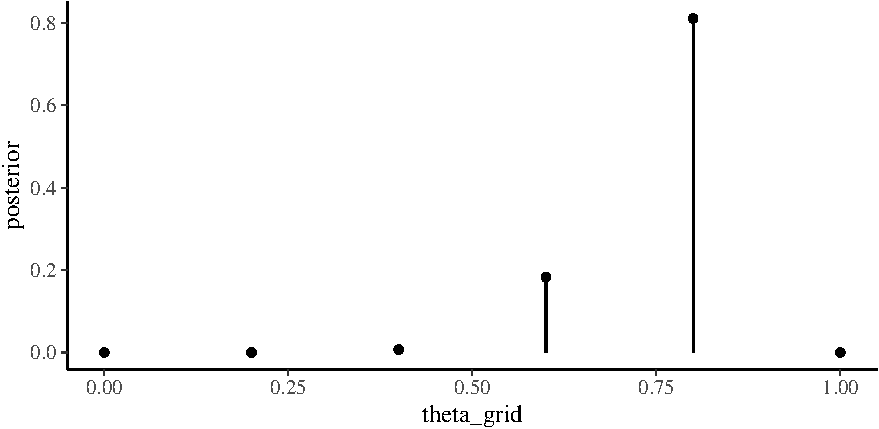
\includegraphics[width=0.8\linewidth]{036_posterior_sim_files/figure-latex/grid-method-6points-posterior-plot-1} 

}

\caption{Distribuzione a posteriori discretizzata ottenuta con il metodo grid-based per $y$ = 9 successi in 10 prove Bernoulliane, con distribuzione a priori $\mbox{Beta}(2, 2)$. È stata utilizzata una griglia di solo $n$ = 6 punti.}\label{fig:grid-method-6points-posterior-plot}
\end{figure}

\noindent
L'ultimo passo della simulazione è il campionamento dalla distribuzione a posteriori discretizzata:

\begin{Shaded}
\begin{Highlighting}[]
\FunctionTok{set.seed}\NormalTok{(}\DecValTok{84735}\NormalTok{)}
\NormalTok{post\_sample }\OtherTok{\textless{}{-}} \FunctionTok{sample\_n}\NormalTok{(}
\NormalTok{  grid\_data,}
  \AttributeTok{size =} \FloatTok{1e5}\NormalTok{,}
  \AttributeTok{weight =}\NormalTok{ posterior,}
  \AttributeTok{replace =} \ConstantTok{TRUE}
\NormalTok{)}
\end{Highlighting}
\end{Shaded}

\noindent
È facile intuire che i valori estratti con rimessa dalla distribuzione a posteriori discretizzata saranno quasi sempre uguali a 0.6 o 0.8. Questa intuizione è confermata dal grafico \ref{fig:grid-method-6points-posterior-plot-sampling} a cui è stata sovrapposta la vera distribuzione a posteriori \(\mbox{Beta}(11, 3)\):

\begin{Shaded}
\begin{Highlighting}[]
\FunctionTok{ggplot}\NormalTok{(post\_sample, }\FunctionTok{aes}\NormalTok{(}\AttributeTok{x =}\NormalTok{ theta\_grid)) }\SpecialCharTok{+}
  \FunctionTok{geom\_histogram}\NormalTok{(}\FunctionTok{aes}\NormalTok{(}\AttributeTok{y =}\NormalTok{ ..density..), }\AttributeTok{color =} \StringTok{"white"}\NormalTok{) }\SpecialCharTok{+}
  \FunctionTok{stat\_function}\NormalTok{(}\AttributeTok{fun =}\NormalTok{ dbeta, }\AttributeTok{args =} \FunctionTok{list}\NormalTok{(}\DecValTok{11}\NormalTok{, }\DecValTok{3}\NormalTok{)) }\SpecialCharTok{+}
  \FunctionTok{lims}\NormalTok{(}\AttributeTok{x =} \FunctionTok{c}\NormalTok{(}\DecValTok{0}\NormalTok{, }\DecValTok{1}\NormalTok{))}
\end{Highlighting}
\end{Shaded}

\begin{figure}[h]

{\centering 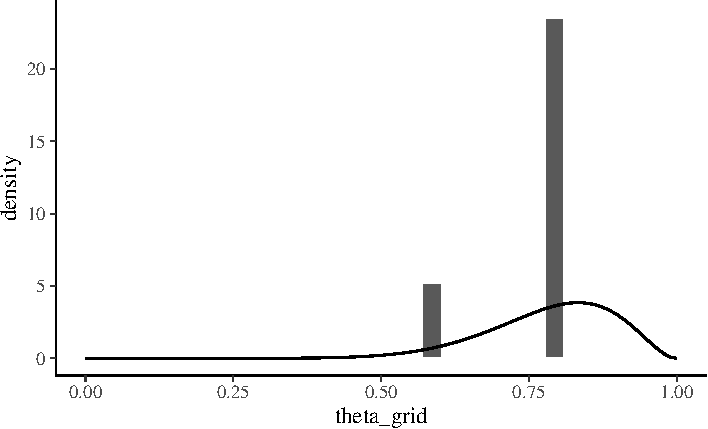
\includegraphics[width=0.8\linewidth]{036_posterior_sim_files/figure-latex/grid-method-6points-posterior-plot-sampling-1} 

}

\caption{Campionamento dalla  distribuzione a posteriori discretizzata ottenuta con il metodo grid-based per $y$ = 9 successi in 10 prove Bernoulliane, con distribuzione a priori $\mbox{Beta}(2, 2)$. È stata utilizzata una griglia di solo $n$ = 6 punti.}\label{fig:grid-method-6points-posterior-plot-sampling}
\end{figure}

\noindent
La figura \ref{fig:grid-method-6points-posterior-plot-sampling} mostra che, con una griglia così sparsa abbiamo ottenuto una versione estremamente approssimata della vera distribuzione a posteriori. Possiamo ottenere un risultato migliore con una griglia più densa, come indicato nella figura \ref{fig:grid-method-100points-posterior-plot-sampling}:

\begin{Shaded}
\begin{Highlighting}[]
\NormalTok{grid\_data  }\OtherTok{\textless{}{-}} \FunctionTok{tibble}\NormalTok{(}
  \AttributeTok{theta\_grid =} \FunctionTok{seq}\NormalTok{(}\AttributeTok{from =} \DecValTok{0}\NormalTok{, }\AttributeTok{to =} \DecValTok{1}\NormalTok{, }\AttributeTok{length.out =} \DecValTok{100}\NormalTok{)}
\NormalTok{)}
\NormalTok{grid\_data }\OtherTok{\textless{}{-}}\NormalTok{ grid\_data }\SpecialCharTok{\%\textgreater{}\%}
  \FunctionTok{mutate}\NormalTok{(}
    \AttributeTok{prior =} \FunctionTok{dbeta}\NormalTok{(theta\_grid, }\DecValTok{2}\NormalTok{, }\DecValTok{2}\NormalTok{),}
    \AttributeTok{likelihood =} \FunctionTok{dbinom}\NormalTok{(}\DecValTok{9}\NormalTok{, }\DecValTok{10}\NormalTok{, theta\_grid)}
\NormalTok{  )}
\NormalTok{grid\_data }\OtherTok{\textless{}{-}}\NormalTok{ grid\_data }\SpecialCharTok{\%\textgreater{}\%}
  \FunctionTok{mutate}\NormalTok{(}
    \AttributeTok{unnormalized =}\NormalTok{ likelihood }\SpecialCharTok{*}\NormalTok{ prior,}
    \AttributeTok{posterior =}\NormalTok{ unnormalized }\SpecialCharTok{/} \FunctionTok{sum}\NormalTok{(unnormalized)}
\NormalTok{  )}
\NormalTok{grid\_data }\SpecialCharTok{\%\textgreater{}\%} 
\FunctionTok{ggplot}\NormalTok{(}
  \FunctionTok{aes}\NormalTok{(}\AttributeTok{x =}\NormalTok{ theta\_grid, }\AttributeTok{y =}\NormalTok{ posterior)}
\NormalTok{) }\SpecialCharTok{+}
  \FunctionTok{geom\_point}\NormalTok{() }\SpecialCharTok{+}
  \FunctionTok{geom\_segment}\NormalTok{(}
    \FunctionTok{aes}\NormalTok{(}
      \AttributeTok{x =}\NormalTok{ theta\_grid, }
      \AttributeTok{xend =}\NormalTok{ theta\_grid, }
      \AttributeTok{y =} \DecValTok{0}\NormalTok{, }
      \AttributeTok{yend =}\NormalTok{ posterior)}
\NormalTok{  )}
\end{Highlighting}
\end{Shaded}

\begin{figure}[h]

{\centering 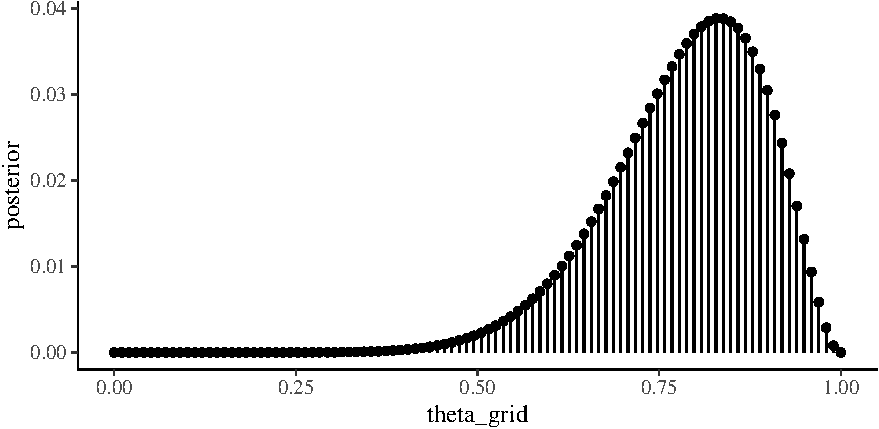
\includegraphics[width=0.8\linewidth]{036_posterior_sim_files/figure-latex/grid-method-100points-posterior-plot-sampling-1} 

}

\caption{Distribuzione a posteriori discretizzata ottenuta con il metodo grid-based per $y$ = 9 successi in 10 prove Bernoulliane, con distribuzione a priori $\mbox{Beta}(2, 2)$. È stata utilizzata una griglia di $n$ = 100 punti.}\label{fig:grid-method-100points-posterior-plot-sampling}
\end{figure}

\noindent
Campioniamo ora 10000 punti:

\begin{Shaded}
\begin{Highlighting}[]
\CommentTok{\# Set the seed}
\FunctionTok{set.seed}\NormalTok{(}\DecValTok{84735}\NormalTok{)}
\NormalTok{post\_sample }\OtherTok{\textless{}{-}} \FunctionTok{sample\_n}\NormalTok{(}
\NormalTok{  grid\_data,}
  \AttributeTok{size =} \FloatTok{1e4}\NormalTok{,}
  \AttributeTok{weight =}\NormalTok{ posterior,}
  \AttributeTok{replace =} \ConstantTok{TRUE}
\NormalTok{)}
\end{Highlighting}
\end{Shaded}

\noindent
Con il campionamento dalla distribuzione a posteriori discretizzata costruita mediante una griglia più densa (\(n = 100\)) otteniamo un risultato soddisfacente (figura \ref{fig:grid-method-100points-posterior-plot-and-correct-posterior}): la distribuzione dei valori prodotti dalla simulazione ora approssima molto bene la corretta distribuzione a posteriori \(p(\theta \mid y) = \mbox{Beta}(11, 3)\).

\begin{Shaded}
\begin{Highlighting}[]
\NormalTok{post\_sample }\SpecialCharTok{\%\textgreater{}\%}
  \FunctionTok{ggplot}\NormalTok{(}\FunctionTok{aes}\NormalTok{(}\AttributeTok{x =}\NormalTok{ theta\_grid)) }\SpecialCharTok{+}
  \FunctionTok{geom\_histogram}\NormalTok{(}
    \FunctionTok{aes}\NormalTok{(}\AttributeTok{y =}\NormalTok{ ..density..), }
    \AttributeTok{color =} \StringTok{"white"}\NormalTok{, }
    \AttributeTok{binwidth =} \FloatTok{0.05}
\NormalTok{  ) }\SpecialCharTok{+}
  \FunctionTok{stat\_function}\NormalTok{(}\AttributeTok{fun =}\NormalTok{ dbeta, }\AttributeTok{args =} \FunctionTok{list}\NormalTok{(}\DecValTok{11}\NormalTok{, }\DecValTok{3}\NormalTok{)) }\SpecialCharTok{+}
  \FunctionTok{lims}\NormalTok{(}\AttributeTok{x =} \FunctionTok{c}\NormalTok{(}\DecValTok{0}\NormalTok{, }\DecValTok{1}\NormalTok{))}
\end{Highlighting}
\end{Shaded}

\begin{figure}[h]

{\centering 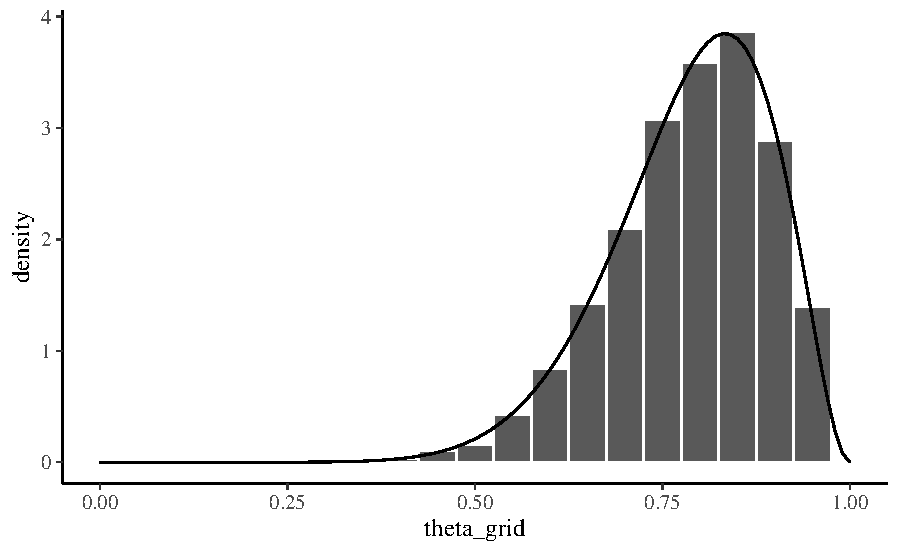
\includegraphics[width=0.8\linewidth]{036_posterior_sim_files/figure-latex/grid-method-100points-posterior-plot-and-correct-posterior-1} 

}

\caption{Campionamento dalla  distribuzione a posteriori discretizzata ottenuta con il metodo grid-based per $y$ = 9 successi in 10 prove Bernoulliane, con distribuzione a priori $\mbox{Beta}(2, 2)$. È stata utilizzata una griglia di $n$ = 100 punti. All'istogramma è stata sovrapposta la corretta distribuzione a posteriori, ovvero la densità $\mbox{Beta}(11, 3)$.}\label{fig:grid-method-100points-posterior-plot-and-correct-posterior}
\end{figure}

Possiamo concludere dicendo che il metodo basato su griglia è molto intuitivo e non richiede particolari competenze di programmazione per essere implementato. Inoltre, fornisce un risultato che, per tutti gli scopi pratici, può essere considerato come un campione casuale estratto da \(p(\theta \mid y)\). Tuttavia, anche se tale metodo fornisce risultati accuratissimi, esso ha un uso limitato. A causa della \emph{maledizione della dimensionalità}\footnote{Che cos'è la \emph{maledizione della dimensionalità}? È molto facile da capire. Supponiamo di utilizzare una griglia di 100 punti equispaziati. Nel caso di un solo parametro, sarà necessario calcolare 100 valori. Per due parametri devono essere calcolari \(100^2\) valori. Ma già per 10 parametri avremo bisogno di calcolare \(10^{10}\) valori -- è facile capire che una tale quantità di calcoli è troppo grande anche per un computer molto potente. Per modelli che richiedono la stima di un numero non piccolo di parametri è dunque necessario procedere in un altro modo.}, infatti, il metodo basato su griglia può essere solo usato nel caso di semplici modelli statistici, con non più di due parametri. Nella pratica concreta tale metodo viene dunque sostituito da altre tecniche più efficienti in quanto, anche nei più comuni modelli utilizzati in psicologia, vengono solitamente stimati centinaia se non migliaia di parametri.

\hypertarget{approssimazione-quadratica}{%
\section{Approssimazione quadratica}\label{approssimazione-quadratica}}

L'approssimazione quadratica è un altro metodo che può essere usato per superare il problema della ``maledizione della dimensionalità''. La motivazione di tale metodo è la seguente. Sappiamo che, in generale, la regione della distribuzione a posteriori che si trova in prossimità del suo massimo può essere ben approssimata dalla forma di una distribuzione Normale.\footnote{Descrivere la distribuzione a posteriori mediante la distribuzione Normale significa utilizzare un'approssimazione che viene, appunto, chiamata ``quadratica'' (tale approssimazione si dice quadratica perché il logaritmo di una distribuzione gaussiana forma una parabola e la parabola è una funzione quadratica -- dunque, mediante questa approssimazione descriviamo il logaritmo della distribuzione a posteriori mediante una parabola).}

L'approssimazione quadratica si pone due obiettivi.

\begin{enumerate}
\def\labelenumi{\arabic{enumi}.}
\tightlist
\item
  Trovare la moda della distribuzione a posteriori. Ci sono varie
  procedure di ottimizzazione, implementate in \(\R\), in
  grado di trovare il massimo di una distribuzione.
\item
  Stimare la curvatura della distribuzione in prossimità della moda.
  Una stima della curvatura è sufficiente per trovare
  un'approssimazione quadratica dell'intera distribuzione. In alcuni
  casi, questi calcoli possono essere fatti seguendo una procedura
  analitica, ma solitamente vengono usate delle tecniche numeriche.
\end{enumerate}

Una descrizione della distribuzione a posteriori ottenuta mediante l'approssimazione quadratica si ottiene mediante la funzione \texttt{quap()} contenuta nel pacchetto \texttt{rethinking}:\footnote{Il pacchetto \texttt{rethinking} è stato creato da \textcite{McElreath_rethinking} per accompagnare il suo testo \emph{Statistical Rethinking}\(^2\). Per l'installazione si veda \url{https://github.com/rmcelreath/rethinking}.}

\begin{Shaded}
\begin{Highlighting}[]
\FunctionTok{suppressPackageStartupMessages}\NormalTok{(}\FunctionTok{library}\NormalTok{(}\StringTok{"rethinking"}\NormalTok{))}

\NormalTok{mod }\OtherTok{\textless{}{-}} \FunctionTok{quap}\NormalTok{(}
  \FunctionTok{alist}\NormalTok{(}
\NormalTok{  N }\SpecialCharTok{\textasciitilde{}} \FunctionTok{dbinom}\NormalTok{(N }\SpecialCharTok{+}\NormalTok{ P, p), }\CommentTok{\# verosimiglianza binomiale}
\NormalTok{  p }\SpecialCharTok{\textasciitilde{}} \FunctionTok{dbeta}\NormalTok{(}\DecValTok{2}\NormalTok{, }\DecValTok{10}\NormalTok{) }\CommentTok{\# distribuzione a priori Beta(2, 10)}
\NormalTok{  ),}
  \AttributeTok{data =} \FunctionTok{list}\NormalTok{(}\AttributeTok{N =} \DecValTok{23}\NormalTok{, }\AttributeTok{P =} \DecValTok{7}\NormalTok{)}
\NormalTok{)}
\end{Highlighting}
\end{Shaded}

Un sommario dell'approssimazione quadratica è fornito da

\begin{Shaded}
\begin{Highlighting}[]
\FunctionTok{precis}\NormalTok{(mod, }\AttributeTok{prob =} \FloatTok{0.95}\NormalTok{)}
\CommentTok{\#\textgreater{}   mean     sd  2.5\% 97.5\%}
\CommentTok{\#\textgreater{} p  0.6 0.0775 0.448 0.752}
\end{Highlighting}
\end{Shaded}

Qui sotto è fornito un confronto tra la corretta distribuzione a posteriori (linea continua) e l'approssimazione quadratica (linea trateggiata).

\begin{Shaded}
\begin{Highlighting}[]
\NormalTok{N }\OtherTok{\textless{}{-}} \DecValTok{23}
\NormalTok{P }\OtherTok{\textless{}{-}} \DecValTok{7}
\NormalTok{a }\OtherTok{\textless{}{-}}\NormalTok{ N }\SpecialCharTok{+} \DecValTok{2}
\NormalTok{b }\OtherTok{\textless{}{-}}\NormalTok{ P }\SpecialCharTok{+} \DecValTok{10}
\FunctionTok{curve}\NormalTok{(}\FunctionTok{dbeta}\NormalTok{(x, a, b), }\AttributeTok{from=}\DecValTok{0}\NormalTok{, }\AttributeTok{to=}\DecValTok{1}\NormalTok{, }\AttributeTok{ylab=}\StringTok{"Densità"}\NormalTok{)}
\CommentTok{\# approssimazione quadratica}
\FunctionTok{curve}\NormalTok{(}
  \FunctionTok{dnorm}\NormalTok{(x, a}\SpecialCharTok{/}\NormalTok{(a}\SpecialCharTok{+}\NormalTok{b), }\FunctionTok{sqrt}\NormalTok{((a}\SpecialCharTok{*}\NormalTok{b)}\SpecialCharTok{/}\NormalTok{((a}\SpecialCharTok{+}\NormalTok{b)}\SpecialCharTok{\^{}}\DecValTok{2}\SpecialCharTok{*}\NormalTok{(a}\SpecialCharTok{+}\NormalTok{b}\SpecialCharTok{+}\DecValTok{1}\NormalTok{)))),}
  \AttributeTok{lty =} \DecValTok{2}\NormalTok{,}
  \AttributeTok{add =} \ConstantTok{TRUE}
\NormalTok{)}
\end{Highlighting}
\end{Shaded}

\begin{center}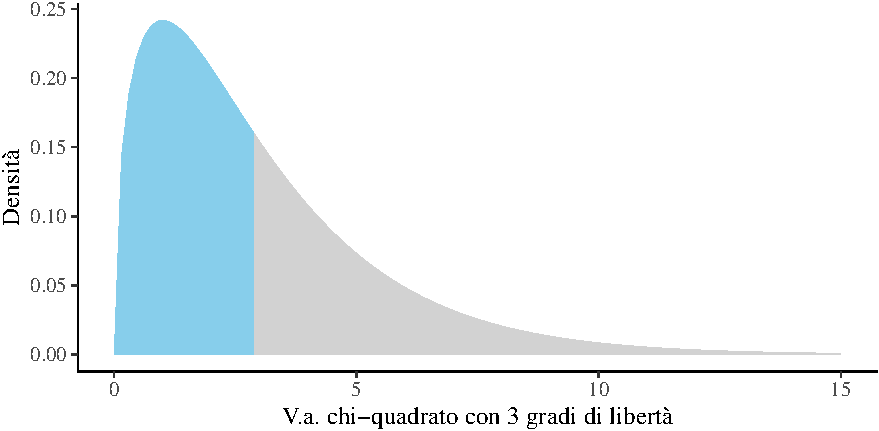
\includegraphics[width=0.8\linewidth]{036_posterior_sim_files/figure-latex/unnamed-chunk-10-1} \end{center}

Il grafico precedente mostra che l'approssimazione quadratica fornisce risultati soddisfacenti. Tali risultati sono simili (o identici) a quelli ottenuti con il metodo \emph{grid-based}, con il vantaggio aggiuntivo di disporre di una serie di funzioni \(\R\) in grado di svolgere i calcoli per noi. In realtà, però, l'approssimazione quadratica è poco usata perché, per problemi complessi, è più conveniente fare ricorso ai metodi Monte Carlo basati su Catena di Markov (MCMC) che verranno descritti nel Paragrafo successivo.

\hypertarget{chapter-simulazioneMC}{%
\section{Metodo Monte Carlo}\label{chapter-simulazioneMC}}

I metodi più ampiamente adottati nell'analisi bayesiana per la costruzione della distribuzione a posteriori per modelli complessi sono i metodi di campionamento detti metodi Monte Carlo basati su catena di Markov (\emph{Markov Chain Monte Carlo}, MCMC). Tali metodi consentono di decidere quali distribuzioni a priori e quali distribuzioni di verosimiglianza usare sulla base di considerazioni teoriche soltanto, senza dovere preoccuparsi di altri vincoli. Dato che è basata su metodi computazionalmente intensivi, la stima numerica MCMC della funzione a posteriori può essere svolta soltanto mediante software. In anni recenti i metodi Bayesiani di analisi dei dati sono diventati sempre più popolari proprio perché la potenza di calcolo necessaria per svolgere tali calcoli è ora alla portata di tutti. Questo non era vero solo pochi decenni fa.

Per introdurre i metodi MCMC consideriamo il caso di una verosimiglianza Binomiale e di una distribuzione a priori Beta. Sappiamo che, in tali circostanze, viene prodotta una distribuzione a posteriori Beta (si veda il capitolo \ref{chapter-distr-coniugate}). Con una simulazione \(\R\) è dunque facile ricavare dei campioni causali dalla distribuzione a posteriori. Maggiore è il numero di campioni, migliore sarà l'approssimazione della distribuzione a posteriori.

Consideriamo nuovamente i dati di \textcite{zetschefuture2019} (23 ``successi'' in 30 prove Bernoulliane) e applichiamo a quei dati lo stesso modello del Capitolo \ref{chapter-distr-coniugate}:
\begin{align}
y \mid \theta, n &\sim \Bin(y = 23, n = 30 \mid \theta) \notag\\
\theta_{prior} &\sim \mbox{Beta}(2, 10) \notag\\
\theta_{post}  &\sim \mbox{Beta}(y + a = 23 + 2 = 25, n - y + b = 30 - 23 + 10 = 17), \notag
\end{align}

\noindent
Poniamoci il problema di stimare il valore della media a posteriori di \(\theta\).
Nel caso presente, il risultato esatto è
\[
\bar{\theta}_{post} = \frac{\alpha}{\alpha + \beta} = \frac{25}{25 + 17} \approx 0.5952.
\]
Dato che la distribuzione a posteriori di \(\theta\) è \(\mbox{Beta}(25, 17)\), possiamo estrarre un campione casuale di osservazioni da tale distribuzione e calcolare la media:

\begin{Shaded}
\begin{Highlighting}[]
\FunctionTok{set.seed}\NormalTok{(}\DecValTok{7543897}\NormalTok{)}
\FunctionTok{print}\NormalTok{(}\FunctionTok{mean}\NormalTok{(}\FunctionTok{rbeta}\NormalTok{(}\FloatTok{1e2}\NormalTok{, }\AttributeTok{shape1 =} \DecValTok{25}\NormalTok{, }\AttributeTok{shape2 =} \DecValTok{17}\NormalTok{)), }\DecValTok{6}\NormalTok{)}
\CommentTok{\#\textgreater{} [1] 0.587548}
\end{Highlighting}
\end{Shaded}

\noindent
È ovvio che l'approssimazione migliora all'aumentare del numero di osservazioni estratte dalla distribuzione a posteriori (legge dei grandi numeri):

\begin{Shaded}
\begin{Highlighting}[]
\FunctionTok{print}\NormalTok{(}\FunctionTok{mean}\NormalTok{(}\FunctionTok{rbeta}\NormalTok{(}\FloatTok{1e3}\NormalTok{, }\AttributeTok{shape1 =} \DecValTok{25}\NormalTok{, }\AttributeTok{shape2 =} \DecValTok{17}\NormalTok{)), }\DecValTok{6}\NormalTok{)}
\CommentTok{\#\textgreater{} [1] 0.597659}
\end{Highlighting}
\end{Shaded}

\begin{Shaded}
\begin{Highlighting}[]
\FunctionTok{print}\NormalTok{(}\FunctionTok{mean}\NormalTok{(}\FunctionTok{rbeta}\NormalTok{(}\FloatTok{1e4}\NormalTok{, }\AttributeTok{shape1 =} \DecValTok{25}\NormalTok{, }\AttributeTok{shape2 =} \DecValTok{17}\NormalTok{)), }\DecValTok{6}\NormalTok{)}
\CommentTok{\#\textgreater{} [1] 0.595723}
\end{Highlighting}
\end{Shaded}

\begin{Shaded}
\begin{Highlighting}[]
\FunctionTok{print}\NormalTok{(}\FunctionTok{mean}\NormalTok{(}\FunctionTok{rbeta}\NormalTok{(}\FloatTok{1e5}\NormalTok{, }\AttributeTok{shape1 =} \DecValTok{25}\NormalTok{, }\AttributeTok{shape2 =} \DecValTok{17}\NormalTok{)), }\DecValTok{6}\NormalTok{)}
\CommentTok{\#\textgreater{} [1] 0.595271}
\end{Highlighting}
\end{Shaded}

\noindent
Quando il numero di osservazioni (possiamo anche chiamarle ``campioni'') tratte dalla distribuzione a posteriori è molto grande, la distribuzione di tali campioni converge alla densità della popolazione (si veda l'Appendice \ref{integration-mc}).\footnote{Si noti, naturalmente, che il numero dei campioni di simulazione è controllato dal ricercatore; è totalmente diverso dalla dimensione del campione che è fissa ed è una proprietà dei dati.}

Inoltre, le statistiche descrittive (es. media, moda, varianza, eccetera) dei campioni estratti dalla distribuzione a posteriori convergeranno ai corrispondenti valori della distribuzione a posteriori. La figura \ref{fig:mcmc-chains-1} mostra come, all'aumentare del numero di repliche, la media, la mediana, la deviazione standard e l'asimmetria convergono ai veri valori della distribuzione a posteriori (linee rosse tratteggiate).

\begin{figure}[h]

{\centering 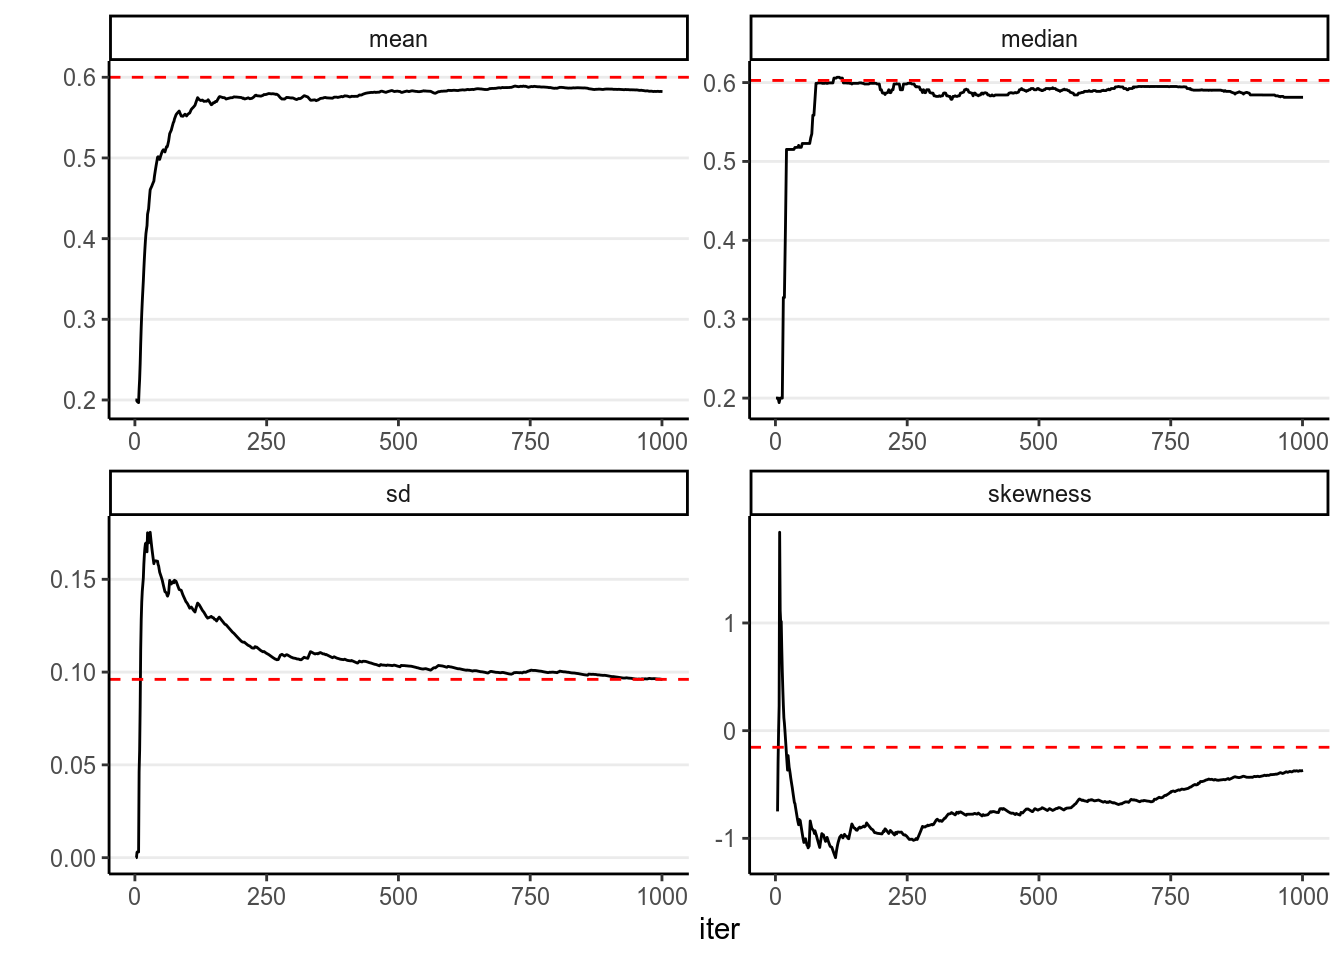
\includegraphics[width=0.8\linewidth]{/Users/corrado/_repositories/dspp/images/mcmc-chains-1} 

}

\caption{Convergenza delle simulazioni Monte Carlo.}\label{fig:mcmc-chains-1}
\end{figure}

\hypertarget{metodi-mc-basati-su-catena-di-markov}{%
\section{Metodi MC basati su Catena di Markov}\label{metodi-mc-basati-su-catena-di-markov}}

Nel Paragrafo \ref{chapter-simulazioneMC} la simulazione Monte Carlo funzionava perché

\begin{itemize}
\tightlist
\item
  sapevamo che la distribuzione a posteriori era una \(\mbox{Beta}(25, 17)\),
\item
  era possibile usare le funzioni \(\R\) per estrarre campioni casuali da tale distribuzione.
\end{itemize}

\noindent
Tuttavia, capita raramente di usare una distribuzione a priori coniugata alla verosimiglianza, quindi in generale le due condizioni descritte sopra non si applicano. Ad esempio, nel caso di una verosimiglianza binomiale e una distribuzione a priori Normale, la distribuzione a posteriori di \(\theta\) è
\[
p(\theta \mid y) = \frac{\mathrm{e}^{-(\theta - 1 / 2)^2} \theta^y (1 - \theta)^{n - y}} {\int_0^1 \mathrm{e}^{-(t - 1 / 2)^2} t^y (1 - t)^{n - y} dt}.
\]
\noindent
Una tale distribuzione non è implementata in \(\R\) e dunque non possiamo campionare da \(p(\theta \mid y)\).

Per fortuna, gli algoritmi MCMC consentono il campionamento da una distribuzione a posteriori \emph{senza che sia necessario conoscere la rappresentazione analitica di una tale distribuzione}. I metodi Monte Carlo basati su catena di Markov consentono di costruire sequenze di punti (detti catene di Markov) nello spazio dei parametri le cui densità sono proporzionali alla distribuzione a posteriori --- in altre parole, dopo aver simulato un grande numero di passi della catena si possono usare i valori così generati come se fossero un campione casuale della distribuzione a posteriori. Le tecniche MCMC sono attualmente il metodo computazionale maggiormente utilizzato per risolvere i problemi di inferenza bayesiana. Un'introduzione alle catene di Markov è fornita nell'Appendice \ref{markov-chains}.

\hypertarget{campionamento-mediante-algoritmi-mcmc}{%
\subsection{Campionamento mediante algoritmi MCMC}\label{campionamento-mediante-algoritmi-mcmc}}

Un modo generale per ottenere una catena di Markov la cui distribuzione equivale alla distribuzione a posteriori \(p(\theta \mid y)\) è quello di usare l'algoritmo di Metropolis. L'algoritmo di Metropolis è il primo algoritmo MCMC che è stato proposto, ed è applicabile ad una grande varietà di problemi inferenziali di tipo bayesiano. Tale algoritmo è stato in seguito sviluppato allo scopo di renderlo via via più efficiente. Lo presentiamo qui in una forma intuitiva.

\hypertarget{una-passeggiata-casuale-sui-numeri-naturali}{%
\subsection{Una passeggiata casuale sui numeri naturali}\label{una-passeggiata-casuale-sui-numeri-naturali}}

Per introdurre l'algoritmo di di Metropolis considereremo il campionamento da una distribuzione discreta.\footnote{Seguiamo qui la trattazione di \textcite{albert2019probability}. Per una presentazione intuitiva dell'algoritmo di Metropolis, si vedano anche \textcite{doing_bayesian_data_an}; \textcite{McElreath_rethinking}.} Supponiamo di definire una distribuzione di probabilità discreta sugli interi \(1,\dots, K\). Scriviamo in \(\R\) la funzione \texttt{pd()} che assegna ai valori \(1,\dots, 8\) delle probabilità proporzionali a 5, 10, 4, 4, 20, 20, 12 e 5.

\begin{Shaded}
\begin{Highlighting}[]
\NormalTok{pd }\OtherTok{\textless{}{-}} \ControlFlowTok{function}\NormalTok{(x)\{}
\NormalTok{  values }\OtherTok{\textless{}{-}} \FunctionTok{c}\NormalTok{(}\DecValTok{5}\NormalTok{, }\DecValTok{10}\NormalTok{, }\DecValTok{4}\NormalTok{, }\DecValTok{4}\NormalTok{, }\DecValTok{20}\NormalTok{, }\DecValTok{20}\NormalTok{, }\DecValTok{12}\NormalTok{, }\DecValTok{5}\NormalTok{)}
  \FunctionTok{ifelse}\NormalTok{(}
\NormalTok{    x }\SpecialCharTok{\%in\%} \DecValTok{1}\SpecialCharTok{:}\FunctionTok{length}\NormalTok{(values),}
\NormalTok{    values[x] }\SpecialCharTok{/} \FunctionTok{sum}\NormalTok{(values),}
    \DecValTok{0}
\NormalTok{  )}
\NormalTok{\}}

\NormalTok{prob\_dist }\OtherTok{\textless{}{-}} \FunctionTok{tibble}\NormalTok{(}
  \AttributeTok{x =} \DecValTok{1}\SpecialCharTok{:}\DecValTok{8}\NormalTok{,}
  \AttributeTok{prob =} \FunctionTok{pd}\NormalTok{(}\DecValTok{1}\SpecialCharTok{:}\DecValTok{8}\NormalTok{)}
\NormalTok{)}
\end{Highlighting}
\end{Shaded}

\noindent
La figura \ref{fig:formetropolisdistr} illustra la distribuzione di probabilità che è stata generata.

\begin{Shaded}
\begin{Highlighting}[]
\NormalTok{x }\OtherTok{\textless{}{-}} \DecValTok{1}\SpecialCharTok{:}\DecValTok{8}
\NormalTok{prob\_dist }\SpecialCharTok{\%\textgreater{}\%}
  \FunctionTok{ggplot}\NormalTok{(}\FunctionTok{aes}\NormalTok{(}\AttributeTok{x =}\NormalTok{ x, }\AttributeTok{y =}\NormalTok{ prob)) }\SpecialCharTok{+}
  \FunctionTok{geom\_bar}\NormalTok{(}\AttributeTok{stat =} \StringTok{"identity"}\NormalTok{, }\AttributeTok{width =} \FloatTok{0.06}\NormalTok{) }\SpecialCharTok{+}
  \FunctionTok{scale\_x\_continuous}\NormalTok{(}\StringTok{"x"}\NormalTok{, }\AttributeTok{labels =} \FunctionTok{as.character}\NormalTok{(x), }\AttributeTok{breaks =}\NormalTok{ x) }\SpecialCharTok{+}
  \FunctionTok{labs}\NormalTok{(}
    \AttributeTok{y =} \StringTok{"Probabilità"}\NormalTok{,}
    \AttributeTok{x =} \StringTok{"X"}
\NormalTok{  )}
\end{Highlighting}
\end{Shaded}

\begin{figure}[h]

{\centering 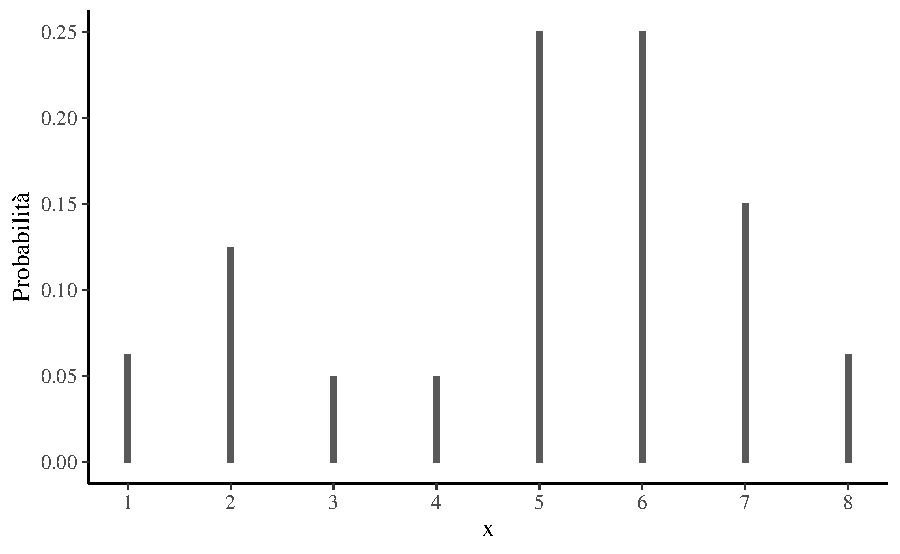
\includegraphics[width=0.8\linewidth]{036_posterior_sim_files/figure-latex/formetropolisdistr-1} 

}

\caption{Distribuzione di massa di probabilità per una variabile casuale avente valori 1, 2, ..., 8.}\label{fig:formetropolisdistr}
\end{figure}

\noindent
L'algoritmo di Metropolis corrisponde alla seguente passeggiata casuale.

\begin{enumerate}
\def\labelenumi{\arabic{enumi}.}
\tightlist
\item
  L'algoritmo inizia con un valore iniziale qualsiasi da 1 a \(K=8\) della variabile casuale.
\item
  Per simulare il valore successivo della sequenza, lanciamo una moneta equilibrata. Se esce testa, consideriamo come valore candidato il valore immediatamente precedente al valore corrente nella sequenza \(1, \dots, 8\); se esce croce, il valore candidato sarà il valore immediatamente successivo al valore corrente nella sequenza.
\item
  Calcoliamo il rapporto tra la probabilità del valore candidato e la probabilità del valore corrente:
  \[
  R = \frac{pd(\text{valore candidato})}{pd(\text{valore corrente})}.
  \]
\item
  Estraiamo un numero a caso \(\in [0, 1]\). Se tale valore è minore di \(R\) accettiamo il valore candidato come valore successivo della catena markoviana; altrimenti il valore successivo della catena rimane il valore corrente.
\end{enumerate}

I passi da 1 a 4 definiscono una catena di Markov irriducibile e aperiodica sui valori di stato \(\{1, 2,\dots, 8\}\), dove il passo 1 fornisce il valore iniziale della catena e i passi da 2 a 4 definiscono la matrice di transizione \(P\). Un modo di campionare da una distribuzione di massa di probabilità \texttt{pd} consiste nell'iniziare da una posizione qualsiasi e eseguire una passeggiata casuale costituita da un grande numero di passi, ripetendo le fasi 2, 3 e 4 dell'algoritmo di Metropolis. Dopo un grande numero di passi, la distribuzione dei valori della catena markoviana approssimerà la distribuzione di probabilità \texttt{pd}.

La funzione \texttt{random\_walk()} implementa l'algoritmo di Metropolis. Tale funzione richiede in input la distribuzione di probabilità \texttt{pd}, la posizione di partenza \texttt{start} e il numero di passi dell'algoritmo \texttt{num\_steps}.

\begin{Shaded}
\begin{Highlighting}[]
\NormalTok{random\_walk }\OtherTok{\textless{}{-}} \ControlFlowTok{function}\NormalTok{(pd, start, num\_steps)\{}
\NormalTok{  y }\OtherTok{\textless{}{-}} \FunctionTok{rep}\NormalTok{(}\DecValTok{0}\NormalTok{, num\_steps)}
\NormalTok{  current }\OtherTok{\textless{}{-}}\NormalTok{ start}
  \ControlFlowTok{for}\NormalTok{ (j }\ControlFlowTok{in} \DecValTok{1}\SpecialCharTok{:}\NormalTok{num\_steps)\{}
\NormalTok{    candidate }\OtherTok{\textless{}{-}}\NormalTok{ current }\SpecialCharTok{+} \FunctionTok{sample}\NormalTok{(}\FunctionTok{c}\NormalTok{(}\SpecialCharTok{{-}}\DecValTok{1}\NormalTok{, }\DecValTok{1}\NormalTok{), }\DecValTok{1}\NormalTok{)}
\NormalTok{    prob }\OtherTok{\textless{}{-}} \FunctionTok{pd}\NormalTok{(candidate) }\SpecialCharTok{/} \FunctionTok{pd}\NormalTok{(current)}
    \ControlFlowTok{if}\NormalTok{ (}\FunctionTok{runif}\NormalTok{(}\DecValTok{1}\NormalTok{) }\SpecialCharTok{\textless{}}\NormalTok{ prob)}
\NormalTok{      current }\OtherTok{\textless{}{-}}\NormalTok{ candidate}
\NormalTok{    y[j] }\OtherTok{\textless{}{-}}\NormalTok{ current}
\NormalTok{  \}}
  \FunctionTok{return}\NormalTok{(y)}
\NormalTok{\}}
\end{Highlighting}
\end{Shaded}

\noindent
Di seguito, implementiamo l'algoritmo di Metropolis utilizzando, quale valore iniziale, \(X=4\). Ripetiamo la simulazione 10,000 volte.

\begin{Shaded}
\begin{Highlighting}[]
\NormalTok{out }\OtherTok{\textless{}{-}} \FunctionTok{random\_walk}\NormalTok{(pd, }\DecValTok{4}\NormalTok{, }\FloatTok{1e4}\NormalTok{)}

\NormalTok{S }\OtherTok{\textless{}{-}} \FunctionTok{tibble}\NormalTok{(out) }\SpecialCharTok{\%\textgreater{}\%}
  \FunctionTok{group\_by}\NormalTok{(out) }\SpecialCharTok{\%\textgreater{}\%}
  \FunctionTok{summarize}\NormalTok{(}
    \AttributeTok{N =} \FunctionTok{n}\NormalTok{(),}
    \AttributeTok{Prob =}\NormalTok{ N }\SpecialCharTok{/} \DecValTok{10000}
\NormalTok{  )}

\NormalTok{prob\_dist2 }\OtherTok{\textless{}{-}} \FunctionTok{rbind}\NormalTok{(}
\NormalTok{  prob\_dist,}
  \FunctionTok{tibble}\NormalTok{(}
    \AttributeTok{x =}\NormalTok{ S}\SpecialCharTok{$}\NormalTok{out,}
    \AttributeTok{prob =}\NormalTok{ S}\SpecialCharTok{$}\NormalTok{Prob}
\NormalTok{    )}
\NormalTok{  )}
\NormalTok{prob\_dist2}\SpecialCharTok{$}\NormalTok{Type }\OtherTok{\textless{}{-}} \FunctionTok{rep}\NormalTok{(}
  \FunctionTok{c}\NormalTok{(}\StringTok{"Prob. corrette"}\NormalTok{, }\StringTok{"Prob. simulate"}\NormalTok{), }
  \AttributeTok{each =} \DecValTok{8}
\NormalTok{  )}
\end{Highlighting}
\end{Shaded}

\begin{Shaded}
\begin{Highlighting}[]
\NormalTok{x }\OtherTok{\textless{}{-}} \DecValTok{1}\SpecialCharTok{:}\DecValTok{8}
\NormalTok{prob\_dist2 }\SpecialCharTok{\%\textgreater{}\%}
  \FunctionTok{ggplot}\NormalTok{(}\FunctionTok{aes}\NormalTok{(}\AttributeTok{x =}\NormalTok{ x, }\AttributeTok{y =}\NormalTok{ prob, }\AttributeTok{fill =}\NormalTok{ Type)) }\SpecialCharTok{+}
  \FunctionTok{geom\_bar}\NormalTok{(}
    \AttributeTok{stat =} \StringTok{"identity"}\NormalTok{, }
    \AttributeTok{width =} \FloatTok{0.1}\NormalTok{, }
    \AttributeTok{position =} \FunctionTok{position\_dodge}\NormalTok{(}\FloatTok{0.3}\NormalTok{)}
\NormalTok{  ) }\SpecialCharTok{+}
  \FunctionTok{scale\_x\_continuous}\NormalTok{(}
    \StringTok{"x"}\NormalTok{, }
    \AttributeTok{labels =} \FunctionTok{as.character}\NormalTok{(x), }
    \AttributeTok{breaks =}\NormalTok{ x}
\NormalTok{  ) }\SpecialCharTok{+}
  \FunctionTok{scale\_fill\_manual}\NormalTok{(}\AttributeTok{values =} \FunctionTok{c}\NormalTok{(}\StringTok{"black"}\NormalTok{, }\StringTok{"gray80"}\NormalTok{)) }\SpecialCharTok{+}
  \FunctionTok{theme}\NormalTok{(}\AttributeTok{legend.title =} \FunctionTok{element\_blank}\NormalTok{()) }\SpecialCharTok{+}
  \FunctionTok{labs}\NormalTok{(}
    \AttributeTok{y =} \StringTok{"Probabilità"}\NormalTok{,}
    \AttributeTok{x =} \StringTok{"X"}
\NormalTok{  )}
\end{Highlighting}
\end{Shaded}

\begin{figure}[h]

{\centering 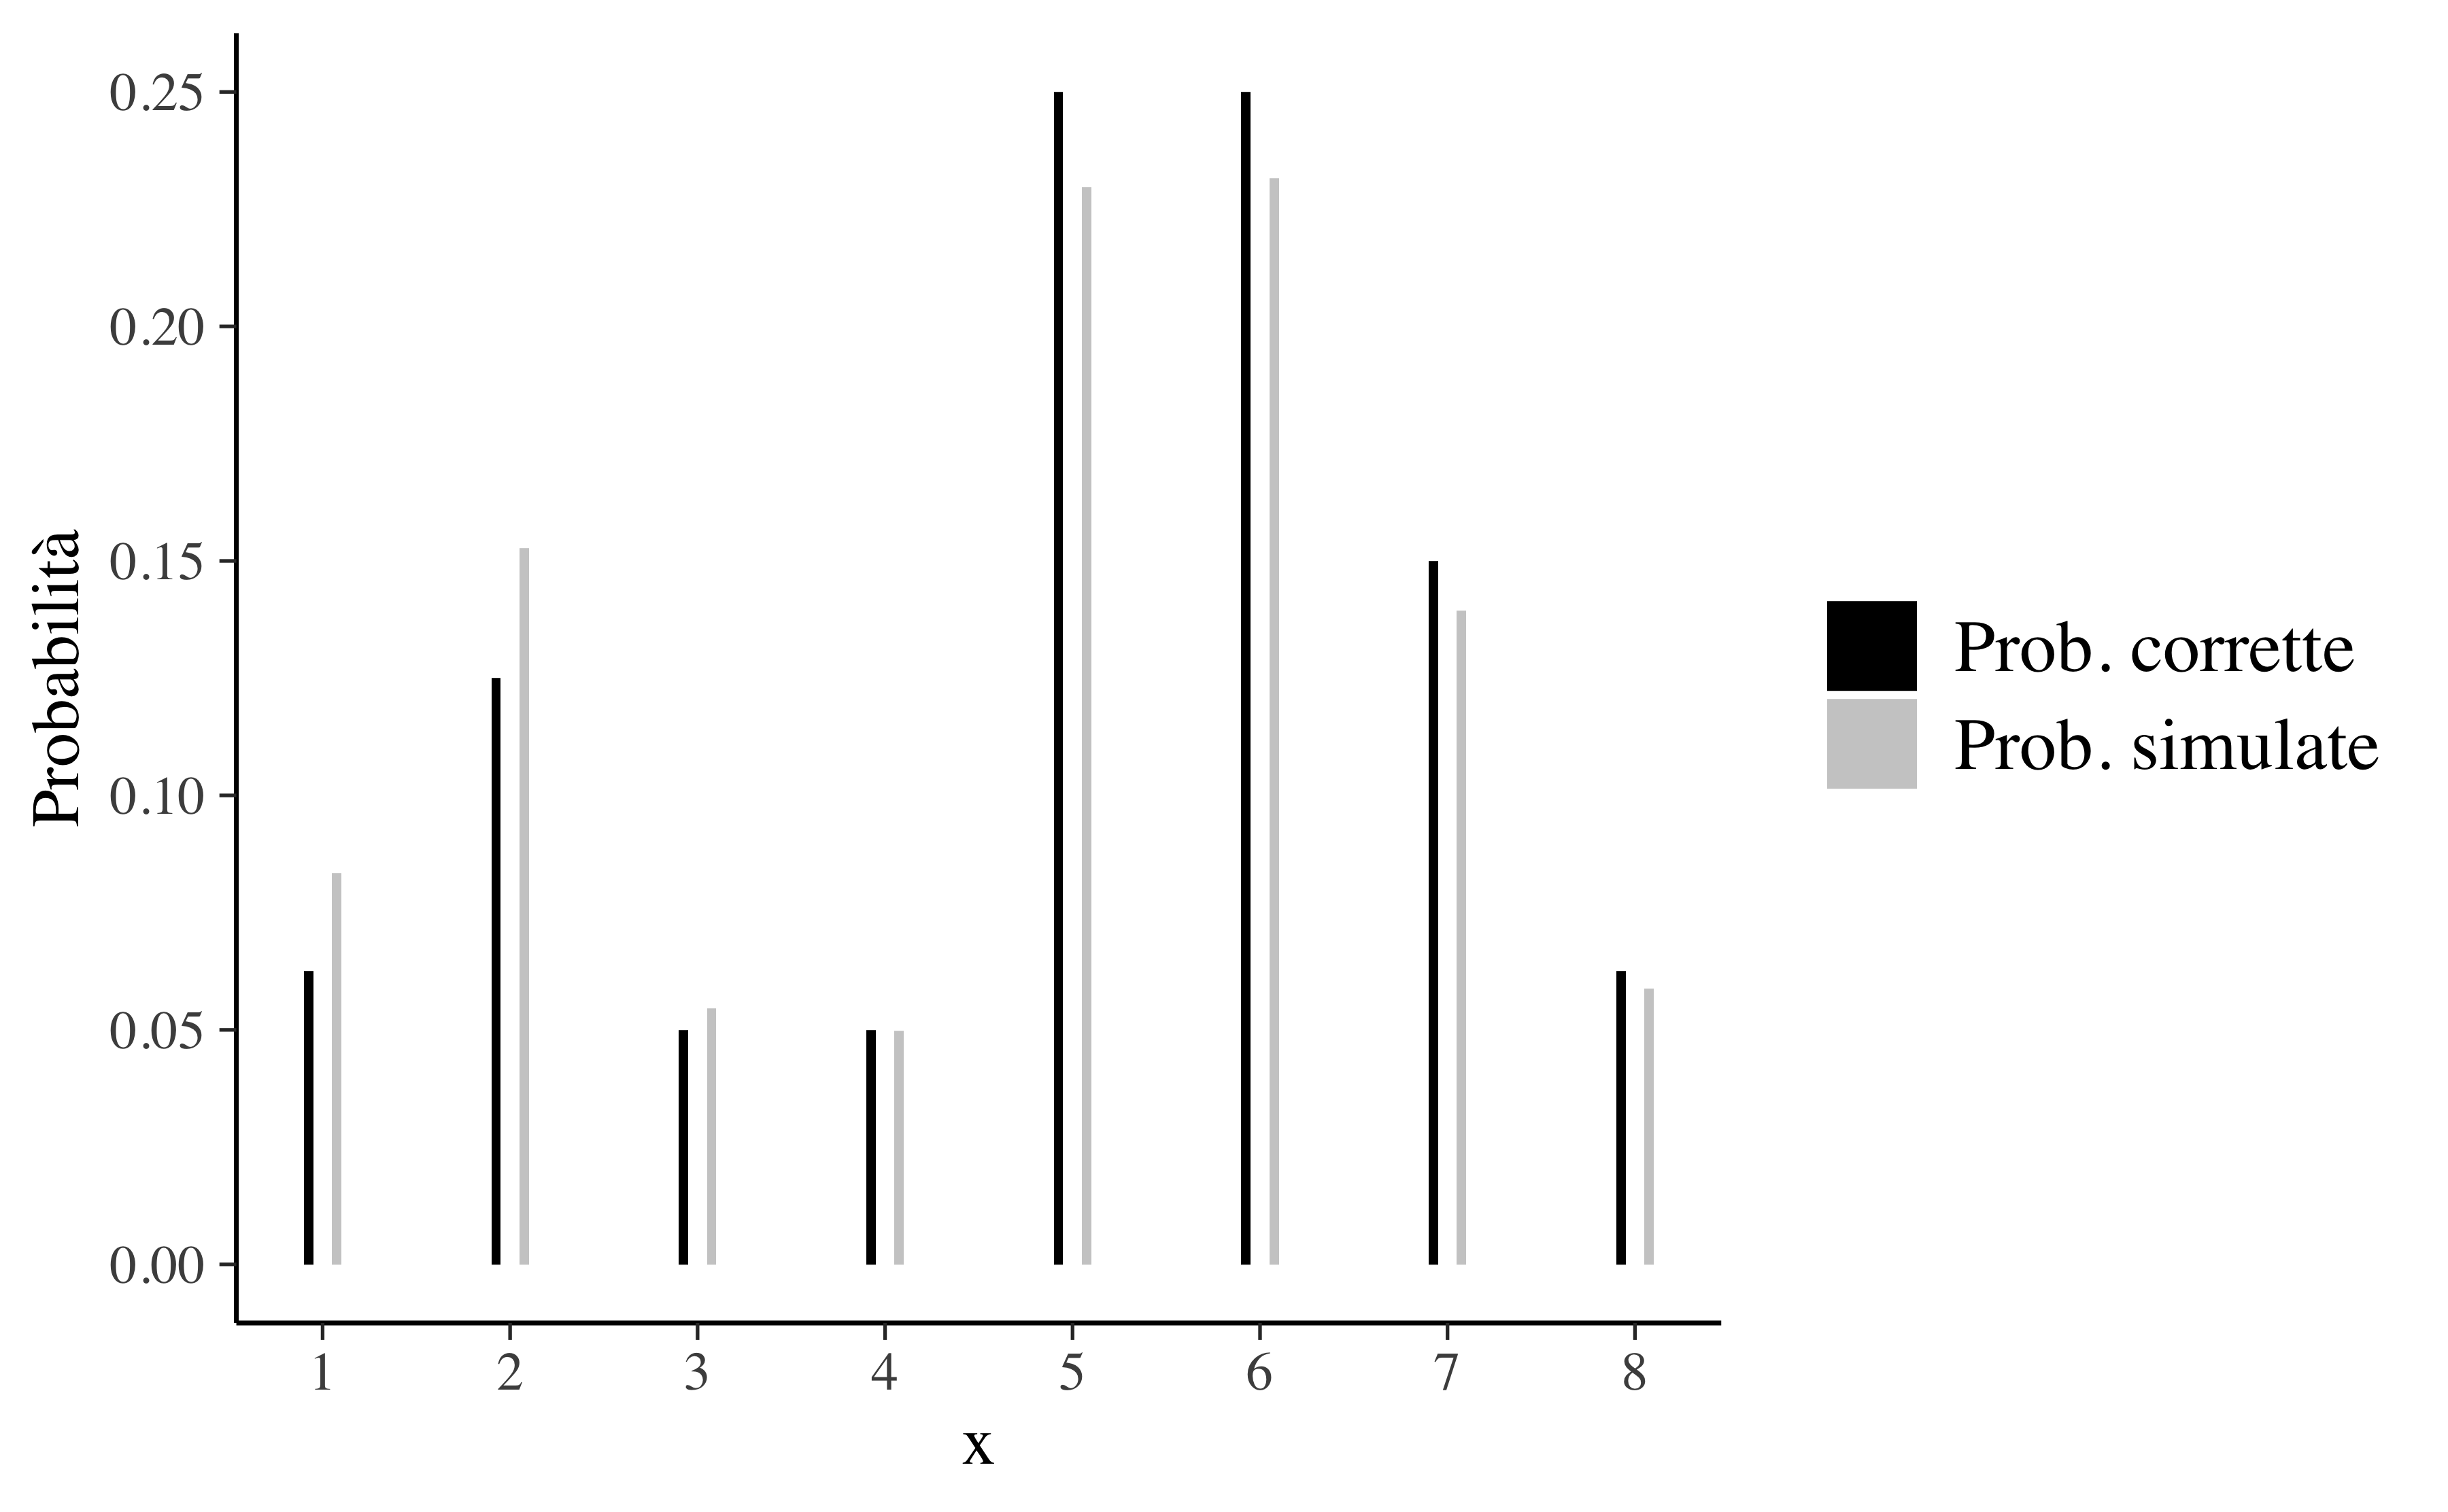
\includegraphics[width=0.8\linewidth]{036_posterior_sim_files/figure-latex/metropolishistogramsim-1} 

}

\caption{L'istogramma confronta i valori prodotti dall'algoritmo di Metropolis con i corretti valori della distribuzione di massa di probabilità.}\label{fig:metropolishistogramsim}
\end{figure}

\noindent
La figura \ref{fig:metropolishistogramsim} confronta l'istogramma dei valori simulati dalla passeggiata casuale con l'effettiva distribuzione di probabilità \texttt{pd}. Si noti la somiglianza tra le due distribuzioni.

\hypertarget{lalgoritmo-di-metropolis}{%
\subsection{L'algoritmo di Metropolis}\label{lalgoritmo-di-metropolis}}

Vediamo ora come l'algoritmo di Metropolis possa venire usato per generare una catena di Markov irriducibile e aperiodica per la quale la distribuzione stazionaria è uguale alla distribuzione a posteriori di interesse.\footnote{Una illustrazione visiva di come si svolge il processo di ``esplorazione'' dell'algoritmo di Metropolis è fornita in questo \href{https://elevanth.org/blog/2017/11/28/build-a-better-markov-chain/}{post}.} In termini generali, l'algoritmo di Metropolis include due fasi.

\begin{itemize}
\tightlist
\item
  \emph{Fase 1.} La selezione di un valore candidato \(\theta'\) del parametro mediante il campionamento da una distribuzione proposta.
\item
  \emph{Fase 2.} La decisione tra la possibilità di accettare il valore candidato \(\theta^{(m+1)} = \theta'\) o di mantenere il valore corrente \(\theta^{(m+1)} = \theta\) sulla base del seguente criterio:

  \begin{itemize}
  \tightlist
  \item
    se \(\mathcal{L}(\theta' \mid y)p(\theta') > \mathcal{L}(\theta \mid y)p(\theta)\) il valore candidato viene sempre accettato;
  \item
    altrimenti il valore candidato viene accettato solo in una certa proporzione di casi.
  \end{itemize}
\end{itemize}

Esaminiamo ora nei dettagli il funzionamento dell'algoritmo di Metropolis.

\begin{enumerate}
\def\labelenumi{(\alph{enumi})}
\item
  Si inizia con un punto arbitrario \(\theta^{(1)}\), quindi il primo valore della catena di Markov \(\theta^{(1)}\) può corrispondere semplicemente ad un valore a caso tra i valori possibili del parametro.
\item
  Per ogni passo successivo della catena, \(m + 1\), si campiona un valore candidato \(\theta'\) da una distribuzione proposta: \(\theta' \sim \Pi(\theta)\). La distribuzione proposta può essere qualunque distribuzione, anche se, idealmente, è meglio che sia simile alla distribuzione a posteriori. In pratica, però, la distribuzione a posteriori è sconosciuta e quindi il valore \(\theta'\) viene campionato da una qualche distribuzione simmetrica centrata sul valore corrente \(\theta^{(m)}\) del parametro. Nell'esempio qui discusso, useremo la distribuzione gaussiana. Tale distribuzione sarà centrata sul valore corrente della catena e avrà una appropriata deviazione standard: \(\theta' \sim \mathcal{N}(\theta^{(m)}, \sigma)\). In pratica, questo significa che, se \(\sigma\) è piccola, il valore candidato \(\theta'\) sarà simile al valore corrente \(\theta^{(m)}\).
\item
  Una volta generato il valore candidato \(\theta'\) si calcola il rapporto tra la densità della distribuzione a posteriori non normalizzata nel punto \(\theta'\) {[}ovvero, il prodotto tra la verosimiglianza \(\mathcal{L}(y \mid \theta')\) nel punto \(\theta'\) e la distribuzione a priori nel punto \(\theta'\){]} e la densità della distribuzione a posteriori non normalizzata nel punto \(\theta^{(m)}\) {[}ovvero, il prodotto tra la verosimiglianza \(\mathcal{L}(y \mid \theta^{(m)})\) nel punto \(\theta^{(m)}\) e la distribuzione a priori nel punto \(\theta^{(m)}\){]}:
  \begin{equation}
  \alpha = \frac{p(y \mid \theta') p(\theta')}{p(y \mid \theta^{(m)}) p(\theta^{(m)})}.
  \label{eq:ratio-metropolis}
  \end{equation}
  \noindent
  Si noti che, essendo un rapporto, la \eqref{eq:ratio-metropolis} cancella la costante di normalizzazione.
\item
  Il rapporto \(\alpha\) viene utilizzato per decidere se accettare il valore candidato \(\theta'\), oppure se campionare un diverso candidato. Possiamo pensare al rapporto \(\alpha\) come alla risposta alla seguente domanda: alla luce dei dati, è più plausibile il valore candidato del parametro o il valore corrente? Se \(\alpha\) è maggiore di 1 ciò significa che il valore candidato è più plausibile del valore corrente; in tali circostanze il valore candidato viene sempre accettato. Altrimenti, si decide di accettare il valore candidato con una probabilità minore di 1, ovvero non sempre, ma soltanto con una probabilità uguale ad \(\alpha\). Se \(\alpha\) è uguale a 0.10, ad esempio, questo significa che la plausibilità a posteriori del valore candidato è 10 volte più piccola della plausibilità a posteriori del valore corrente. Dunque, il valore candidato verrà accettato solo nel 10\% dei casi. Come conseguenza di questa strategia di scelta, l'algoritmo di Metropolis ottiene un campione casuale dalla distribuzione a posteriori, dato che la probabilità di accettare il valore candidato è proporzionale alla densità del candidato nella distribuzione a posteriori. Dal punto di vista algoritmico, la procedura descritta sopra viene implementata confrontando il rapporto \(\alpha\) con un valore casuale estratto da una distribuzione uniforme \(\mbox{Unif}(0, 1)\). Se \(\alpha > u \sim \mbox{Unif}(0, 1)\) allora il punto candidato \(\theta'\) viene accettato e la catena si muove in quella nuova posizione, ovvero \(\theta^{(m+1)} = \theta'^{(m+1)}\). Altrimenti \(\theta^{(m+1)} = \theta^{(m)}\) e si campiona un nuovo valore candidato \(\theta'\).
\item
  Il passaggio finale dell'algoritmo calcola l'\emph{accettanza} in una specifica esecuzione dell'algoritmo, ovvero la proporzione dei valori candidati \(\theta'\) che sono stati accettati come valori successivi nella sequenza.
\end{enumerate}

L'algoritmo di Metropolis prende come input il numero \(M\) di passi da simulare, la deviazione standard \(\sigma\) della distribuzione proposta e la densità a priori, e ritorna come output la sequenza \(\theta^{(1)}, \theta^{(2)}, \dots, \theta^{(M)}\). La chiave del successo dell'algoritmo di Metropolis è il numero di passi fino a che la catena approssima la stazionarietà. Tipicamente i primi da 1000 a 5000 elementi sono scartati. Dopo un certo periodo \(k\) (detto di \emph{burn-in}), la catena di Markov converge ad una variabile casuale che è distribuita secondo la distribuzione a posteriori. In altre parole, i campioni del vettore \(\left(\theta^{(k+1)}, \theta^{(k+2)}, \dots, \theta^{(M)}\right)\) diventano campioni di \(p(\theta \mid y)\).

\hypertarget{una-applicazione-concreta}{%
\subsection{Una applicazione concreta}\label{una-applicazione-concreta}}

Per fare un esempio concreto, consideriamo nuovamente i 30 pazienti esaminati da \textcite{zetschefuture2019}. Di essi, 23 hanno manifestato aspettative distorte negativamente sul loro stato d'animo futuro. Utilizzando l'algoritmo di Metropolis, ci poniamo il problema di ottenere la stima a posteriori di \(\theta\) (probabilità di manifestare un'aspettativa distorta negativamente), dati 23 ``successi'' in 30 prove, imponendo su \(\theta\) la stessa distribuzione a priori usata nel Capitolo \ref{chapter-distr-coniugate}, ovvero \(\mbox{Beta}(2, 10)\).

Per calcolare la funzione di verosimiglianza, avendo fissato i dati di \textcite{zetschefuture2019}, definiamo la funzione \texttt{likelihood()}

\begin{Shaded}
\begin{Highlighting}[]
\NormalTok{likelihood }\OtherTok{\textless{}{-}} \ControlFlowTok{function}\NormalTok{(param, }\AttributeTok{x =} \DecValTok{23}\NormalTok{, }\AttributeTok{N =} \DecValTok{30}\NormalTok{) \{}
  \FunctionTok{dbinom}\NormalTok{(x, N, param)}
\NormalTok{\}}
\end{Highlighting}
\end{Shaded}

\noindent
che ritorna l'ordinata della verosimiglianza binomiale per ciascun valore del vettore \texttt{param} in input.

La distribuzione a priori \(\mbox{Beta}(2, 10)\) è implementata nella funzione \texttt{prior()}:

\begin{Shaded}
\begin{Highlighting}[]
\NormalTok{prior }\OtherTok{\textless{}{-}} \ControlFlowTok{function}\NormalTok{(param, }\AttributeTok{alpha =} \DecValTok{2}\NormalTok{, }\AttributeTok{beta =} \DecValTok{10}\NormalTok{) \{}
  \FunctionTok{dbeta}\NormalTok{(param, alpha, beta) }
\NormalTok{\}}
\end{Highlighting}
\end{Shaded}

Il prodotto della densità a priori e della verosimiglianza è implementato nella funzione \texttt{posterior()}:

\begin{Shaded}
\begin{Highlighting}[]
\NormalTok{posterior }\OtherTok{\textless{}{-}} \ControlFlowTok{function}\NormalTok{(param) \{}
  \FunctionTok{likelihood}\NormalTok{(param) }\SpecialCharTok{*} \FunctionTok{prior}\NormalTok{(param)}
\NormalTok{\}}
\end{Highlighting}
\end{Shaded}

L'Appendice \ref{es-pratico-zetsche-funzioni} mostra come un'approssimazione della distribuzione a posteriori \(p(\theta \mid y)\) per questi dati possa essere ottenuta mediante il metodo basato su griglia.

\hypertarget{implementazione}{%
\subsection{Implementazione}\label{implementazione}}

Per implementare l'algoritmo di Metropolis utilizzeremo una distribuzione proposta gaussiana. Il valore candidato sarà dunque un valore selezionato a caso da una gaussiana di parametri \(\mu\) uguale al valore corrente nella catena e \(\sigma = 0.9\). In questo esempio, la deviazione standard \(\sigma\) è stata scelta empiricamente in modo tale da ottenere una accettanza adeguata. L'accettanza ottimale è di circa 0.20 e 0.30 --- se l'accettanza è troppo grande, l'algoritmo esplora uno spazio troppo ristretto della distribuzione a posteriori.\footnote{L'accettanza dipende dalla distribuzione proposta: in generale, tanto più la distribuzione proposta è simile alla distribuzione target, tanto più alta diventa l'accettanza.}

\begin{Shaded}
\begin{Highlighting}[]
\NormalTok{proposal\_distribution }\OtherTok{\textless{}{-}} \ControlFlowTok{function}\NormalTok{(param) \{}
  \ControlFlowTok{while}\NormalTok{(}\DecValTok{1}\NormalTok{) \{}
\NormalTok{    res }\OtherTok{=} \FunctionTok{rnorm}\NormalTok{(}\DecValTok{1}\NormalTok{, }\AttributeTok{mean =}\NormalTok{ param, }\AttributeTok{sd =} \FloatTok{0.9}\NormalTok{)}
    \ControlFlowTok{if}\NormalTok{ (res }\SpecialCharTok{\textgreater{}} \DecValTok{0} \SpecialCharTok{\&}\NormalTok{ res }\SpecialCharTok{\textless{}} \DecValTok{1}\NormalTok{)}
      \ControlFlowTok{break}
\NormalTok{  \}}
\NormalTok{  res}
\NormalTok{\}}
\end{Highlighting}
\end{Shaded}

\noindent 
Nella presente implementazione del campionamento dalla distribuzione proposta è stato inserito un controllo che impone al valore candidato di essere incluso nell'intervallo {[}0, 1{]}.\footnote{Si possono trovare implementazioni dell'algoritmo di Metropolis più eleganti di quella presentata qui. Lo scopo dell'esercizio è quello di illustrare la logica soggiacente all'algoritmo di Metropolis, non quello di proporre un'implementazione efficente dell'algoritmo.}

L'algoritmo di Metropolis viene implementato nella seguente funzione:

\begin{Shaded}
\begin{Highlighting}[]
\NormalTok{run\_metropolis\_MCMC }\OtherTok{\textless{}{-}} \ControlFlowTok{function}\NormalTok{(startvalue, iterations) \{}
\NormalTok{  chain }\OtherTok{\textless{}{-}} \FunctionTok{vector}\NormalTok{(}\AttributeTok{length =}\NormalTok{ iterations }\SpecialCharTok{+} \DecValTok{1}\NormalTok{)}
\NormalTok{  chain[}\DecValTok{1}\NormalTok{] }\OtherTok{\textless{}{-}}\NormalTok{ startvalue}
  \ControlFlowTok{for}\NormalTok{ (i }\ControlFlowTok{in} \DecValTok{1}\SpecialCharTok{:}\NormalTok{iterations) \{}
\NormalTok{    proposal }\OtherTok{\textless{}{-}} \FunctionTok{proposal\_distribution}\NormalTok{(chain[i])}
\NormalTok{    r }\OtherTok{\textless{}{-}} \FunctionTok{posterior}\NormalTok{(proposal) }\SpecialCharTok{/} \FunctionTok{posterior}\NormalTok{(chain[i])}
    \ControlFlowTok{if}\NormalTok{ (}\FunctionTok{runif}\NormalTok{(}\DecValTok{1}\NormalTok{) }\SpecialCharTok{\textless{}}\NormalTok{ r) \{}
\NormalTok{      chain[i }\SpecialCharTok{+} \DecValTok{1}\NormalTok{] }\OtherTok{\textless{}{-}}\NormalTok{ proposal}
\NormalTok{    \} }\ControlFlowTok{else}\NormalTok{ \{}
\NormalTok{      chain[i }\SpecialCharTok{+} \DecValTok{1}\NormalTok{] }\OtherTok{\textless{}{-}}\NormalTok{ chain[i]}
\NormalTok{    \}}
\NormalTok{  \}}
\NormalTok{  chain}
\NormalTok{\}}
\end{Highlighting}
\end{Shaded}

Avendo definito le funzioni precedenti, generiamo una catena di valori \(\theta\):

\begin{Shaded}
\begin{Highlighting}[]
\FunctionTok{set.seed}\NormalTok{(}\DecValTok{123}\NormalTok{)}
\NormalTok{startvalue }\OtherTok{\textless{}{-}} \FunctionTok{runif}\NormalTok{(}\DecValTok{1}\NormalTok{, }\DecValTok{0}\NormalTok{, }\DecValTok{1}\NormalTok{)}
\NormalTok{niter }\OtherTok{\textless{}{-}} \FloatTok{1e4}
\NormalTok{chain }\OtherTok{\textless{}{-}} \FunctionTok{run\_metropolis\_MCMC}\NormalTok{(startvalue, niter)}
\end{Highlighting}
\end{Shaded}

Mediante le istruzioni precedenti otteniamo una catena di Markov costituita da 10,001 valori. Escludiamo i primi 5,000 valori considerati come burn-in. Ci restano dunque con 5,001 valori che verranno considerati come un campione casuale estratto dalla distribuzione a posteriori \(p(\theta \mid y)\).

L'accettanza è pari a

\begin{Shaded}
\begin{Highlighting}[]
\NormalTok{burnIn }\OtherTok{\textless{}{-}}\NormalTok{ niter }\SpecialCharTok{/} \DecValTok{2}
\NormalTok{acceptance }\OtherTok{\textless{}{-}} \DecValTok{1} \SpecialCharTok{{-}} \FunctionTok{mean}\NormalTok{(}\FunctionTok{duplicated}\NormalTok{(chain[}\SpecialCharTok{{-}}\NormalTok{(}\DecValTok{1}\SpecialCharTok{:}\NormalTok{burnIn)]))}
\NormalTok{acceptance}
\CommentTok{\#\textgreater{} [1] 0.251}
\end{Highlighting}
\end{Shaded}

\noindent
il che conferma la bontà della deviazione standard (\(\sigma\) = 0.9) scelta per la distribuzione proposta.

A questo punto è facile ottenere una stima a posteriori del parametro \(\theta\). Per esempio, la stima della media a posteriori è:

\begin{Shaded}
\begin{Highlighting}[]
\FunctionTok{mean}\NormalTok{(chain[}\SpecialCharTok{{-}}\NormalTok{(}\DecValTok{1}\SpecialCharTok{:}\NormalTok{burnIn)])}
\CommentTok{\#\textgreater{} [1] 0.592}
\end{Highlighting}
\end{Shaded}

Una figura che mostra l'approssimazione di \(p(\theta \mid y)\) ottenuta con l'algoritmo di Metropolis, insieme ad un \emph{trace plot} dei valori della catena di Markov, viene prodotta usando le seguenti istruzioni:

\begin{Shaded}
\begin{Highlighting}[]
\NormalTok{p1 }\OtherTok{\textless{}{-}} \FunctionTok{tibble}\NormalTok{(}
  \AttributeTok{x =}\NormalTok{ chain[}\SpecialCharTok{{-}}\NormalTok{(}\DecValTok{1}\SpecialCharTok{:}\NormalTok{burnIn)]}
\NormalTok{  ) }\SpecialCharTok{\%\textgreater{}\%}
  \FunctionTok{ggplot}\NormalTok{(}\FunctionTok{aes}\NormalTok{(x)) }\SpecialCharTok{+}
  \FunctionTok{geom\_histogram}\NormalTok{() }\SpecialCharTok{+}
  \FunctionTok{labs}\NormalTok{(}
    \AttributeTok{x =} \FunctionTok{expression}\NormalTok{(theta),}
    \AttributeTok{y =} \StringTok{"Frequenza"}\NormalTok{,}
    \AttributeTok{title =} \StringTok{"Distribuzione a posteriori"}
\NormalTok{  ) }\SpecialCharTok{+}
  \FunctionTok{geom\_vline}\NormalTok{(}
    \AttributeTok{xintercept =} \FunctionTok{mean}\NormalTok{(chain[}\SpecialCharTok{{-}}\NormalTok{(}\DecValTok{1}\SpecialCharTok{:}\NormalTok{burnIn)])}
\NormalTok{  )}
\NormalTok{p2 }\OtherTok{\textless{}{-}} \FunctionTok{tibble}\NormalTok{(}
  \AttributeTok{x =} \DecValTok{1}\SpecialCharTok{:}\FunctionTok{length}\NormalTok{(chain[}\SpecialCharTok{{-}}\NormalTok{(}\DecValTok{1}\SpecialCharTok{:}\NormalTok{burnIn)]),}
  \AttributeTok{y =}\NormalTok{ chain[}\SpecialCharTok{{-}}\NormalTok{(}\DecValTok{1}\SpecialCharTok{:}\NormalTok{burnIn)]}
\NormalTok{  ) }\SpecialCharTok{\%\textgreater{}\%}
  \FunctionTok{ggplot}\NormalTok{(}\FunctionTok{aes}\NormalTok{(x, y)) }\SpecialCharTok{+}
  \FunctionTok{geom\_line}\NormalTok{() }\SpecialCharTok{+}
  \FunctionTok{labs}\NormalTok{(}
    \AttributeTok{x =} \StringTok{"Numero di passi"}\NormalTok{,}
    \AttributeTok{y =} \FunctionTok{expression}\NormalTok{(theta),}
    \AttributeTok{title =} \StringTok{"Valori della catena"}
\NormalTok{  ) }\SpecialCharTok{+}
  \FunctionTok{geom\_hline}\NormalTok{(}
    \AttributeTok{yintercept =} \FunctionTok{mean}\NormalTok{(chain[}\SpecialCharTok{{-}}\NormalTok{(}\DecValTok{1}\SpecialCharTok{:}\NormalTok{burnIn)]),}
    \AttributeTok{colour =} \StringTok{"gray"}
\NormalTok{  )}
\NormalTok{p1 }\SpecialCharTok{+}\NormalTok{ p2}
\end{Highlighting}
\end{Shaded}

\begin{figure}[h]

{\centering 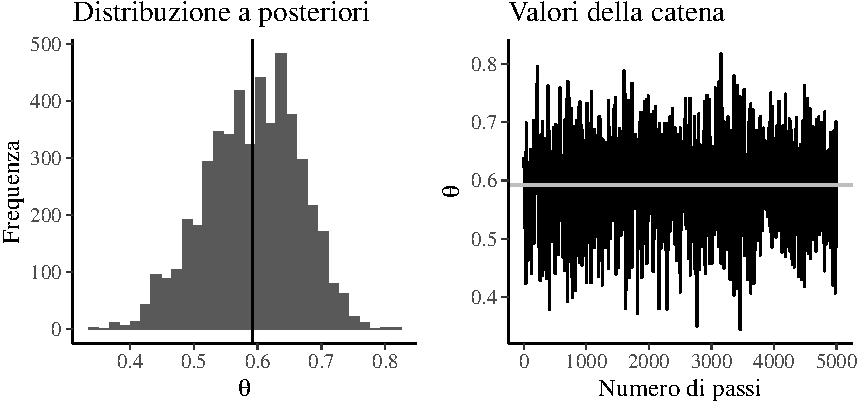
\includegraphics[width=0.8\linewidth]{036_posterior_sim_files/figure-latex/sim-markov-chain-zetsche-1} 

}

\caption{Sinistra. Stima della distribuzione a posteriori della probabilità di una aspettativa futura distorta negativamente per i dati di Zetsche et al. (2019). Destra. Trace plot dei valori della catena di Markov escludendo il periodo di burn-in.}\label{fig:sim-markov-chain-zetsche}
\end{figure}

\hypertarget{input}{%
\subsection{Input}\label{input}}

Negli esempi discussi in questo Capitolo abbiamo illustrato l'esecuzione di una singola catena in cui si parte un unico valore iniziale e si raccolgono i valori simulati da molte iterazioni. È possibile che i valori di una catena siano influenzati dalla scelta del valore iniziale. Quindi una raccomandazione generale è di eseguire l'algoritmo di Metropolis più volte utilizzando diversi valori di partenza. In questo caso, si avranno più catene di Markov. Confrontando le proprietà delle diverse catene si esplora la sensibilità dell'inferenza alla scelta del valore di partenza. I software MCMC consentono sempre all'utente di specificare diversi valori di partenza e di generare molteplici catene di Markov.

\hypertarget{stazionarietuxe0}{%
\section{Stazionarietà}\label{stazionarietuxe0}}

Un punto importante da verificare è se il campionatore ha raggiunto la sua distribuzione stazionaria. La convergenza di una catena di Markov alla distribuzione stazionaria viene detta ``mixing''.

\hypertarget{approx-post-autocor}{%
\subsection{Autocorrelazione}\label{approx-post-autocor}}

Informazioni sul ``mixing'' della catena di Markov sono fornite dall'autocorrelazione. L'autocorrelazione misura la correlazione tra i valori successivi di una catena di Markov. Il valore \(m\)-esimo della serie ordinata viene confrontato con un altro valore ritardato di una quantità \(k\) (dove \(k\) è l'entità del ritardo) per verificare quanto si correli al variare di \(k\). L'autocorrelazione di ordine 1 (\emph{lag 1}) misura la correlazione tra valori successivi della catena di Markow (cioè, la correlazione tra \(\theta^{(m)}\) e \(\theta^{(m-1)}\)); l'autocorrelazione di ordine 2 (\emph{lag 2}) misura la correlazione tra valori della catena di Markow separati da due ``passi'' (cioè, la correlazione tra \(\theta^{(m)}\) e \(\theta^{(m-2)}\)); e così via.

L'autocorrelazione di ordine \(k\) è data da \(\rho_k\) e può essere stimata come:
\begin{align}
\rho_k &= \frac{\Cov(\theta_m, \theta_{m+k})}{\Var(\theta_m)}\notag\\
&= \frac{\sum_{m=1}^{n-k}(\theta_m - \bar{\theta})(\theta_{m-k} - \bar{\theta})}{\sum_{m=1}^{n-k}(\theta_m - \bar{\theta})^2} \qquad\text{con }\quad \bar{\theta} = \frac{1}{n}\sum_{m=1}^{n}\theta_m.
\label{eq:autocor}
\end{align}
Per fare un esempio pratico, simuliamo dei dati autocorrelati con la funzione R \texttt{colorednoise::colored\_noise()}:

\begin{Shaded}
\begin{Highlighting}[]
\FunctionTok{suppressPackageStartupMessages}\NormalTok{(}\FunctionTok{library}\NormalTok{(}\StringTok{"colorednoise"}\NormalTok{))}
\FunctionTok{set.seed}\NormalTok{(}\DecValTok{34783859}\NormalTok{)}
\NormalTok{rednoise }\OtherTok{\textless{}{-}} \FunctionTok{colored\_noise}\NormalTok{(}
  \AttributeTok{timesteps =} \DecValTok{30}\NormalTok{, }\AttributeTok{mean =} \FloatTok{0.5}\NormalTok{, }\AttributeTok{sd =} \FloatTok{0.05}\NormalTok{, }\AttributeTok{phi =} \FloatTok{0.3}
\NormalTok{)}
\end{Highlighting}
\end{Shaded}

L'autocorrelazione di ordine 1 è semplicemente la correlazione tra ciascun elemento e quello successivo nella sequenza. Nell'esempio, il vettore \texttt{rednoise} è una sequenza temporale di 30 elementi. Il vettore \texttt{rednoise{[}-length(rednoise){]}} include gli elementi con gli indici da 1 a 29 nella sequenza originaria, mentre il vettore \texttt{rednoise{[}-1{]}} include gli elementi 2:30. Gli elementi delle coppie ordinate dei due vettori avranno dunque gli indici \((1, 2), (2, 3), \dots (29, 30)\) degli elementi della sequenza originaria. La correlazione di Pearson tra i vettori \texttt{rednoise{[}-length(rednoise){]}} e \texttt{rednoise{[}-1{]}} corrisponde dunque all'autocorrelazione di ordine 1 della serie temporale.

\begin{Shaded}
\begin{Highlighting}[]
\FunctionTok{cor}\NormalTok{(rednoise[}\SpecialCharTok{{-}}\FunctionTok{length}\NormalTok{(rednoise)], rednoise[}\SpecialCharTok{{-}}\DecValTok{1}\NormalTok{])}
\CommentTok{\#\textgreater{} [1] 0.397}
\end{Highlighting}
\end{Shaded}

Il Correlogramma è uno strumento grafico usato per la valutazione della tendenza di una catena di Markov nel tempo. Il correlogramma si costruisce a partire dall'autocorrelazione \(\rho_k\) di una catena di Markov in funzione del ritardo (\emph{lag}) \(k\) con cui l'autocorrelazione è calcolata: nel grafico ogni barretta verticale riporta il valore dell'autocorrelazione (sull'asse delle ordinate) in funzione del ritardo (sull'asse delle ascisse). In \(\R\), il correlogramma può essere prodotto con una chiamata a \texttt{acf()}:

\begin{Shaded}
\begin{Highlighting}[]
\FunctionTok{acf}\NormalTok{(rednoise)}
\end{Highlighting}
\end{Shaded}

\begin{center}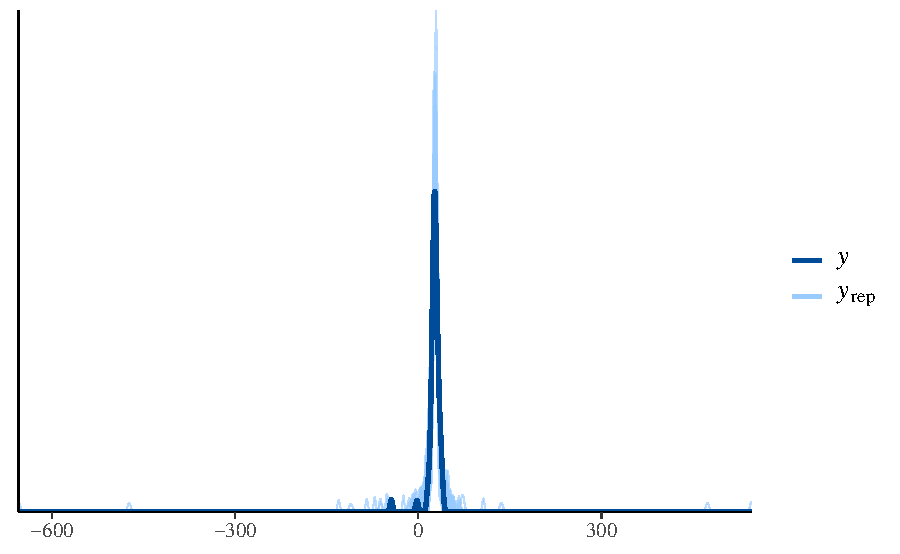
\includegraphics[width=0.8\linewidth]{036_posterior_sim_files/figure-latex/unnamed-chunk-28-1} \end{center}

Il correlogramma precedente mostra come l'autocorrelazione di ordine 1 sia circa pari a 0.4 e diminuisce per lag maggiori; per lag di 4, l'autocorrelazione diventa negativa e aumenta progressivamente fino ad un lag di 8; eccetera.

In situazioni ottimali l'autocorrelazione diminuisce rapidamente ed è effettivamente pari a 0 per piccoli lag. Ciò indica che i valori della catena di Markov che si trovano a più di soli pochi passi di distanza gli uni dagli altri non risultano associati tra loro, il che fornisce conferma del ``mixing'' della catena di Markov, ossia di convergenza alla distribuzione stazionaria.
Nelle analisi bayesiane, una delle strategie che consentono di ridurre l'autocorrelazione è quella di assottigliare l'output immagazzinando solo ogni \(m\)-esimo punto dopo il periodo di burn-in. Una tale strategia va sotto il nome di \emph{thinning}.

\hypertarget{test-di-convergenza}{%
\subsection{Test di convergenza}\label{test-di-convergenza}}

Un test di convergenza può essere svolto in maniera grafica mediante le tracce delle serie temporali (\emph{trace plot}), cioè il grafico dei valori simulati rispetto al numero di iterazioni. Se la catena è in uno stato stazionario le tracce mostrano assenza di periodicità nel tempo e ampiezza costante, senza tendenze visibili o andamenti degni di nota. Un esempio di \emph{trace plot} è fornito nella figura \ref{fig:sim-markov-chain-zetsche} (destra).

Ci sono inoltre alcuni test che permettono di verificare la stazionarietà del campionatore dopo un dato punto. Uno è il test di Geweke che suddivide il campione, dopo aver rimosso un periodo di burn in, in due parti. Se la catena è in uno stato stazionario, le medie dei due campioni dovrebbero essere uguali. Un test modificato, chiamato Geweke z-score, utilizza un test \(z\) per confrontare i due subcampioni ed il risultante test statistico, se ad esempio è più alto di 2, indica che la media della serie sta ancora muovendosi da un punto ad un altro e quindi è necessario un periodo di burn-in più lungo.

\hypertarget{considerazioni-conclusive}{%
\section*{Considerazioni conclusive}\label{considerazioni-conclusive}}
\addcontentsline{toc}{section}{Considerazioni conclusive}

In generale, la distribuzione a posteriori dei parametri di un modello statistico non può essere determinata per via analitica. Tale problema, invece, viene affrontato facendo ricorso ad una classe di algoritmi per il campionamento da distribuzioni di probabilità che sono estremamente onerosi dal punto di vista computazionale e che possono essere utilizzati nelle applicazioni pratiche solo grazie alla potenza di calcolo dei moderni computer. Lo sviluppo di software che rendono sempre più semplice l'uso dei metodi MCMC, insieme all'incremento della potenza di calcolo dei computer, ha contribuito a rendere sempre più popolare il metodo dell'inferenza bayesiana che, in questo modo, può essere estesa a problemi di qualunque grado di complessità.

Nel 1989 un gruppo di statistici nel Regno Unito si pose il problema di simulare le catene di Markov su un personal computer. Nel 1997 ci riuscirono con il primo rilascio pubblico di un'implementazione Windows dell'inferenza bayesiana basata su Gibbs sampling, detta BUGS. Il materiale presentato in questo capitolo descrive gli sviluppi contemporanei del percorso che è iniziato in quel periodo.

\hypertarget{appendix-appendix}{%
\appendix}


\hypertarget{markov-chains}{%
\chapter{Le catene di Markov}\label{markov-chains}}

Per introdurre il concetto di catena di Markov, supponiamo che una persona esegua una passeggiata casuale sulla retta dei numeri naturali considerando solo i valori 1, 2, 3, 4, 5, 6.\footnote{Seguiamo qui la presentazione fornita da \href{https://github.com/bob-carpenter/prob-stats}{Bob Carpenter}.} Se la persona è collocata su un valore interno dei valori possibili (ovvero, 2, 3, 4 o 5), nel passo successivo è altrettanto probabile che rimanga su quel numero o si sposti su un numero adiacente. Se si muove, è ugualmente probabile che si muova a sinistra o a destra. Se la persona si trova su uno dei valori estremi (ovvero, 1 o 6), nel passo successivo è altrettanto probabile che rimanga rimanga su quel numero o si sposti nella posizione adiacente.

Questo è un esempio di una catena di Markov discreta. Una catena di Markov descrive il movimento probabilistico tra un numero di stati. Nell'esempio ci sono sei possibili stati, da 1 a 6, i quali corrispondono alle possibili posizioni della passeggiata casuale. Data la sua posizione corrente, la persona si sposterà nelle altre posizioni possibili con delle specifiche probabilità. La probabilità che si sposti in un'altra posizione dipende solo dalla sua posizione attuale e non dalle posizioni visitate in precedenza.

È possibile descrivere il movimento tra gli stati nei termini delle cosiddette \emph{probabilità di transizione}, ovvero le probabilità di movimento tra tutti i possibili stati in un unico passaggio di una catena di Markov. Le probabilità di transizione sono riassunte in una \emph{matrice di transizione} \(P\):

\begin{Shaded}
\begin{Highlighting}[]
\NormalTok{p }\OtherTok{\textless{}{-}} \FunctionTok{c}\NormalTok{(}\DecValTok{0}\NormalTok{, }\DecValTok{0}\NormalTok{, }\DecValTok{1}\NormalTok{, }\DecValTok{0}\NormalTok{, }\DecValTok{0}\NormalTok{, }\DecValTok{0}\NormalTok{)}

\NormalTok{P }\OtherTok{\textless{}{-}} \FunctionTok{matrix}\NormalTok{(}
  \FunctionTok{c}\NormalTok{(.}\DecValTok{5}\NormalTok{, .}\DecValTok{5}\NormalTok{, }\DecValTok{0}\NormalTok{, }\DecValTok{0}\NormalTok{, }\DecValTok{0}\NormalTok{, }\DecValTok{0}\NormalTok{,}
\NormalTok{    .}\DecValTok{25}\NormalTok{, .}\DecValTok{5}\NormalTok{, .}\DecValTok{25}\NormalTok{, }\DecValTok{0}\NormalTok{, }\DecValTok{0}\NormalTok{, }\DecValTok{0}\NormalTok{,}
    \DecValTok{0}\NormalTok{, .}\DecValTok{25}\NormalTok{, .}\DecValTok{5}\NormalTok{, .}\DecValTok{25}\NormalTok{, }\DecValTok{0}\NormalTok{, }\DecValTok{0}\NormalTok{,}
    \DecValTok{0}\NormalTok{, }\DecValTok{0}\NormalTok{, .}\DecValTok{25}\NormalTok{, .}\DecValTok{5}\NormalTok{, .}\DecValTok{25}\NormalTok{, }\DecValTok{0}\NormalTok{,}
    \DecValTok{0}\NormalTok{, }\DecValTok{0}\NormalTok{, }\DecValTok{0}\NormalTok{, .}\DecValTok{25}\NormalTok{, .}\DecValTok{5}\NormalTok{, .}\DecValTok{25}\NormalTok{,}
    \DecValTok{0}\NormalTok{, }\DecValTok{0}\NormalTok{, }\DecValTok{0}\NormalTok{, }\DecValTok{0}\NormalTok{, .}\DecValTok{5}\NormalTok{, .}\DecValTok{5}
\NormalTok{    ),}
  \AttributeTok{nrow =} \DecValTok{6}\NormalTok{, }\AttributeTok{ncol =} \DecValTok{6}\NormalTok{, }\AttributeTok{byrow =} \ConstantTok{TRUE}\NormalTok{)}

\NormalTok{kableExtra}\SpecialCharTok{::}\FunctionTok{kable}\NormalTok{(P)}
\end{Highlighting}
\end{Shaded}

\begin{tabular}{r|r|r|r|r|r}
\hline
0.50 & 0.50 & 0.00 & 0.00 & 0.00 & 0.00\\
\hline
0.25 & 0.50 & 0.25 & 0.00 & 0.00 & 0.00\\
\hline
0.00 & 0.25 & 0.50 & 0.25 & 0.00 & 0.00\\
\hline
0.00 & 0.00 & 0.25 & 0.50 & 0.25 & 0.00\\
\hline
0.00 & 0.00 & 0.00 & 0.25 & 0.50 & 0.25\\
\hline
0.00 & 0.00 & 0.00 & 0.00 & 0.50 & 0.50\\
\hline
\end{tabular}

\hfill\break

La prima riga della matrice di transizione \(P\) fornisce le probabilità di passare a ciascuno degli stati da 1 a 6 in un unico passaggio a partire dalla posizione 1; la seconda riga fornisce le probabilità di transizione in un unico passaggio dalla posizione 2 e così via. Per esempio, il valore \(P[1, 1]\) ci dice che, se la persona è nello stato 1, avrà una probabilità di 0.5 di rimanere in quello stato; \(P[1, 2]\) ci dice che c'è una probabilità di 0.5 di passare dallo stato 1 allo stato 2. Gli altri elementi della prima riga sono 0 perché, in un unico passaggio, non è possibile passare dallo stato 1 agli stati 3, 4, 5 e 6. Il valore \(P[2, 1]\) ci dice che, se la persona è nello stato 1 (seconda riga), avrà una probabilità di 0.25 di passare allo stato 1; avra una probabilità di 0.5 di rimanere in quello stato, \(P[2, 2]\); e avrà una probabilità di 0.25 di passare allo stato 3, \(P[2, 3]\); eccetera.

Si notino alcune importanti proprietà di questa particolare catena di Markov.

\begin{itemize}
\tightlist
\item
  È possibile passare da ogni stato a qualunque altro stato in uno o più passaggi: una catena di Markov con questa proprietà si dice \emph{irriducibile}.
\item
  Dato che la persona si trova in un particolare stato, se può tornare a questo stato solo a intervalli regolari, si dice che la catena di Markov è \emph{periodica}. In questo esempio la catena è \emph{aperiodica} poiché la passeggiata casuale non può eitornare allo stato attuale a intervalli regolari.
\end{itemize}

Un'importante proprietà di una catena di Markov irriducibile e aperiodica è che il passaggio ad uno stato del sistema dipende unicamente dallo stato immediatamente precedente e non dal come si è giunti a tale stato (dalla storia). Per questo motivo si dice che un processo markoviano è senza memoria. Tale ``assenza di memoria'' può essere interpretata come la proprietà mediante cui è possibile ottenere un insieme di campioni casuali da una distribuzione di interesse. Nel caso dell'inferenza bayesiana, la distribuzione di interesse è la distribuzione a posteriori, \(p(\theta \mid y)\). Le catene di Markov consentono di stimare i valori di aspettazione di variabili rispetto alla distribuzione a posteriori.

La matrice di transizione che si ottiene dopo un enorme numero di passi di una passeggiata casuale markoviana si chiama \emph{distribuzione stazionaria}. Se una catena di Markov è irriducibile e aperiodica, allora ha un'unica distribuzione stazionaria \(w\). La distribuzione limite di una tale catena di Markov, quando il numero di passi tende all'infinito, è uguale alla distribuzione stazionaria \(w\).

\hypertarget{simulare-una-catena-di-markov}{%
\section{Simulare una catena di Markov}\label{simulare-una-catena-di-markov}}

Un metodo per dimostrare l'esistenza della distribuzione stazionaria di una catena di Markov è quello di eseguire un esperimento di simulazione. Iniziamo una passeggiata casuale partendo da un particolare stato, diciamo la posizione 3, e quindi simuliamo molti passaggi della catena di Markov usando la matrice di transizione \(P\). Al crescere del numero di passi della catena, le frequenze relative che descrivono il passaggio a ciascuno dei sei possibili nodi della catena approssimano sempre meglio la distribuzione stazionaria \(w\).

Senza entrare nei dettagli della simulazione, la figura \ref{fig:markovsim} mostra i risultati ottenuti in 10,000 passi di una passeggiata casuale markoviana. Si noti che, all'aumentare del numero di iterazioni, le frequenze relative approssimano sempre meglio le probabilità nella distribuzione stazionaria \(w = (0.1, 0.2, 0.2, 0.2, 0.2, 0.1)\).

\begin{Shaded}
\begin{Highlighting}[]
\FunctionTok{set.seed}\NormalTok{(}\DecValTok{123}\NormalTok{)}
\NormalTok{s }\OtherTok{\textless{}{-}} \FunctionTok{vector}\NormalTok{(}\StringTok{"numeric"}\NormalTok{, }\DecValTok{10000}\NormalTok{)}
\NormalTok{s[}\DecValTok{1}\NormalTok{] }\OtherTok{\textless{}{-}} \DecValTok{3}
\ControlFlowTok{for}\NormalTok{ (j }\ControlFlowTok{in} \DecValTok{2}\SpecialCharTok{:}\DecValTok{10000}\NormalTok{)\{}
\NormalTok{  s[j] }\OtherTok{\textless{}{-}} \FunctionTok{sample}\NormalTok{(}\DecValTok{1}\SpecialCharTok{:}\DecValTok{6}\NormalTok{, }\AttributeTok{size=}\DecValTok{1}\NormalTok{, }\AttributeTok{prob=}\NormalTok{P[s[j }\SpecialCharTok{{-}} \DecValTok{1}\NormalTok{], ])}
\NormalTok{\}}
\NormalTok{S }\OtherTok{\textless{}{-}} \FunctionTok{data.frame}\NormalTok{(}\AttributeTok{Iterazione =} \DecValTok{1}\SpecialCharTok{:}\DecValTok{10000}\NormalTok{,}
                \AttributeTok{Location =}\NormalTok{ s)}

\NormalTok{S }\SpecialCharTok{\%\textgreater{}\%} \FunctionTok{mutate}\NormalTok{(}\AttributeTok{L1 =}\NormalTok{ (Location }\SpecialCharTok{==} \DecValTok{1}\NormalTok{),}
             \AttributeTok{L2 =}\NormalTok{ (Location }\SpecialCharTok{==} \DecValTok{2}\NormalTok{),}
             \AttributeTok{L3 =}\NormalTok{ (Location }\SpecialCharTok{==} \DecValTok{3}\NormalTok{),}
             \AttributeTok{L4 =}\NormalTok{ (Location }\SpecialCharTok{==} \DecValTok{4}\NormalTok{),}
             \AttributeTok{L5 =}\NormalTok{ (Location }\SpecialCharTok{==} \DecValTok{5}\NormalTok{),}
             \AttributeTok{L6 =}\NormalTok{ (Location }\SpecialCharTok{==} \DecValTok{6}\NormalTok{))  }\SpecialCharTok{\%\textgreater{}\%}
  \FunctionTok{mutate}\NormalTok{(}\AttributeTok{Proporzione\_1 =} \FunctionTok{cumsum}\NormalTok{(L1) }\SpecialCharTok{/}\NormalTok{ Iterazione,}
         \AttributeTok{Proporzione\_2 =} \FunctionTok{cumsum}\NormalTok{(L2) }\SpecialCharTok{/}\NormalTok{ Iterazione,}
         \AttributeTok{Proporzione\_3 =} \FunctionTok{cumsum}\NormalTok{(L3) }\SpecialCharTok{/}\NormalTok{ Iterazione,}
         \AttributeTok{Proporzione\_4 =} \FunctionTok{cumsum}\NormalTok{(L4) }\SpecialCharTok{/}\NormalTok{ Iterazione,}
         \AttributeTok{Proporzione\_5 =} \FunctionTok{cumsum}\NormalTok{(L5) }\SpecialCharTok{/}\NormalTok{ Iterazione,}
         \AttributeTok{Proporzione\_6 =} \FunctionTok{cumsum}\NormalTok{(L6) }\SpecialCharTok{/}\NormalTok{ Iterazione) }\SpecialCharTok{\%\textgreater{}\%}
  \FunctionTok{select}\NormalTok{(Iterazione, Proporzione\_1, Proporzione\_2, Proporzione\_3,}
\NormalTok{         Proporzione\_4, Proporzione\_5, Proporzione\_6) }\OtherTok{{-}\textgreater{}}\NormalTok{ S1}

\FunctionTok{gather}\NormalTok{(S1, Outcome, Probability, }\SpecialCharTok{{-}}\NormalTok{Iterazione) }\OtherTok{{-}\textgreater{}}\NormalTok{ S2}

\FunctionTok{ggplot}\NormalTok{(S2, }\FunctionTok{aes}\NormalTok{(Iterazione, Probability)) }\SpecialCharTok{+}
  \FunctionTok{geom\_line}\NormalTok{() }\SpecialCharTok{+}
  \FunctionTok{facet\_wrap}\NormalTok{(}\SpecialCharTok{\textasciitilde{}}\NormalTok{ Outcome, }\AttributeTok{ncol =} \DecValTok{3}\NormalTok{) }\SpecialCharTok{+}
  \FunctionTok{ylim}\NormalTok{(}\DecValTok{0}\NormalTok{, .}\DecValTok{4}\NormalTok{) }\SpecialCharTok{+}
  \FunctionTok{ylab}\NormalTok{(}\StringTok{"Frequenza relativa"}\NormalTok{) }\SpecialCharTok{+}
  \CommentTok{\# theme(text=element\_text(size=14))  +}
  \FunctionTok{scale\_x\_continuous}\NormalTok{(}\AttributeTok{breaks =} \FunctionTok{c}\NormalTok{(}\DecValTok{0}\NormalTok{, }\DecValTok{3000}\NormalTok{, }\DecValTok{6000}\NormalTok{, }\DecValTok{9000}\NormalTok{))}
\end{Highlighting}
\end{Shaded}

\begin{figure}[h]

{\centering 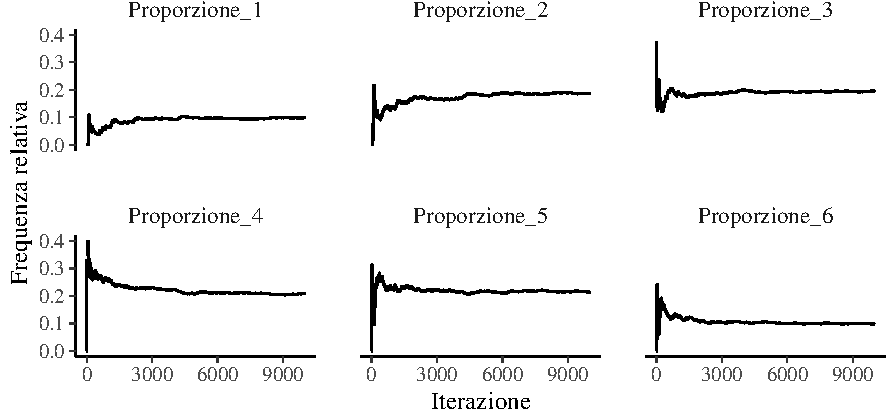
\includegraphics[width=0.8\linewidth]{913_markov_chains_files/figure-latex/markovsim-1} 

}

\caption{Frequenze relative degli stati da 1 a 6 in funzione del numero di iterazioni per la simulazione di una catena di Markov.}\label{fig:markovsim}
\end{figure}

Il metodo di campionamento utilizzato dagli algoritmi MCMC consente di creare una catena di Markov irriducibile e aperiodica, la cui distribuzione stazionaria equivale alla distribuzione a posteriori \(p(\theta \mid y)\).


% Bibliography
%%%%%%%%%%%%%%%%%%%%%%%%%%%%%%%%%%%%%%%%%%%%%%%%%%%%%%%%%%

\backmatter
\SmallMargins

\printbibliography
\onecolumn


% Tables (of tables, of figures)
%%%%%%%%%%%%%%%%%%%%%%%%%%%%%%%%%%%%%%%%%%%%%%%%%%%%%%%%%%


\cleardoublepage
\LargeMargins
\listoffigures


% After-body (LaTeX code inclusion)
%%%%%%%%%%%%%%%%%%%%%%%%%%%%%%%%%%%%%%%%%%%%%%%%%%%%%%%%%%




% Back cover
%%%%%%%%%%%%%%%%%%%%%%%%%%%%%%%%%%%%%%%%%%%%%%%%%%%%%%%%%%%

% Even page, small margins, no running head, no page number.
\evenpage
\SmallMargins
\thispagestyle{empty}

\begin{normalsize}

\begin{description}

\selectlanguage{italian}
\item[Abstract]
This document contains the material of the lessons of Psicometria B000286 (2021/2022) aimed at students of the first year of the Degree Course in Psychological Sciences and Techniques of the University of Florence, Italy.
\item[Keywords]
Data science, Bayesian statistics.
~\\

\end{description}

\end{normalsize}


\end{document}
